% !TeX spellcheck = pt_BR
% ------------------------------------------------------------------------
% ------------------------------------------------------------------------
% abnTeX2: Modelo de Trabalho Academico (tese de doutorado, dissertacao de
% mestrado e trabalhos monograficos em geral) em conformidade com 
% ABNT NBR 14724:2011: Informacao e documentacao - Trabalhos academicos -
% Apresentacao
% ------------------------------------------------------------------------
% ------------------------------------------------------------------------

\documentclass[
    % -- opções da classe memoir --
    12pt,               % tamanho da fonte
    openright,          % capítulos começam em pág ímpar (insere página vazia caso preciso)
    oneside,
    %twoside,           % para impressão em recto e verso. Oposto a oneside
    a4paper,            % tamanho do papel. 
    % -- opções da classe abntex2 --
    %chapter=TITLE,     % títulos de capítulos convertidos em letras maiúsculas
    %section=TITLE,     % títulos de seções convertidos em letras maiúsculas
    %subsection=TITLE,  % títulos de subseções convertidos em letras maiúsculas
    %subsubsection=TITLE,% títulos de subsubseções convertidos em letras maiúsculas
    % -- opções do pacote babel --
    english,            % idioma adicional para hifenização
    french,             % idioma adicional para hifenização
    spanish,            % idioma adicional para hifenização
    brazil              % o último idioma é o principal do documento
    ]{abntex2}

% ---
% Pacotes básicos 
% ---
\usepackage[utf8]{inputenc}
\usepackage{lmodern}            % Usa a fonte Latin Modern          
\usepackage[T1]{fontenc}        % Selecao de codigos de fonte.

\usepackage{lastpage}           % Usado pela Ficha catalográfica
\usepackage{indentfirst}        % Indenta o primeiro parágrafo de cada seção.
\usepackage{color}              % Controle das cores
\usepackage{graphicx}           % Inclusão de gráficos
\usepackage{microtype}          % para melhorias de justificação
\usepackage{longtable}          % para tabelas longas
\usepackage{tabularx,ragged2e}
\usepackage{multirow}
\usepackage{algpseudocode,algorithm}    % para algoritmos       
\usepackage{pdfpages}
\usepackage{subfig}
\usepackage{hyperref}
\usepackage{amsmath}
%\usepackage{subcaption}
% ---
        
% ---
% Pacotes adicionais, usados apenas no âmbito do Modelo Canônico do abnteX2
% ---
\usepackage{lipsum}             % para geração de dummy text
% ---

% ---
% Pacotes de citações
% ---
\usepackage[brazilian,hyperpageref]{backref}     % Paginas com as citações na bibl
\usepackage[alf]{abntex2cite}   % Citações padrão ABNT


%Espaçamento em formulas e tabelas
\renewcommand{\arraystretch}{1.3}
\newcommand{\matlab}{MATLAB\textsuperscript{\textregistered}}

% Please add the following required packages to your document preamble:
\usepackage{multirow}
\usepackage[table,xcdraw]{xcolor}
% If you use beamer only pass "xcolor=table" option, i.e. \documentclass[xcolor=table]{beamer}

% --- 
% CONFIGURAÇÕES DE PACOTES
% --- 

% ---
% Configurações do pacote backref
% Usado sem a opção hyperpageref de backref
\renewcommand{\backrefpagesname}{Citado na(s) página(s):~}
% Texto padrão antes do número das páginas
\renewcommand{\backref}{}
% Define os textos da citação
\renewcommand*{\backrefalt}[4]{
    \ifcase #1 %
        Nenhuma citação no texto.%
    \or
        Citado na página #2.%
    \else
        Citado #1 vezes nas páginas #2.%
    \fi}%
% ---

% ---
% Informações de dados para CAPA e FOLHA DE ROSTO
% ---
\titulo{Avaliação quantitativa do método do gradiente conjugado precondicionado para a solução paralela e concorrente de um modelo de elementos finitos}
\autor{Thiago de Sousa Goveia}
\local{Timóteo}
\data{2017}
\orientador{Márcio Matias}
\instituicao{%
    Centro Federal de Educação Tecnológica de Minas Gerais
    \par
    Campus Timóteo
    \par
    Graduação em Engenharia de Computação
}
\tipotrabalho{Trabalho de conclusão de curso I (Graduação)}

% O preambulo deve conter o tipo do trabalho, o objetivo, 
% o nome da instituição e a área de concentração 
\preambulo{Proposta de trabalho apresentada como requisito das disciplinas trabalho de conclusão de curso I  e metodologia de pesquisa.}
% ---


% ---
% Configurações de aparência do PDF final

% alterando o aspecto da cor azul
\definecolor{blue}{RGB}{41,5,195}

% informações do PDF
\makeatletter
\hypersetup{
        %pagebackref=true,
        pdftitle={\@title}, 
        pdfauthor={\@author},
        pdfsubject={\imprimirpreambulo},
        pdfcreator={LaTeX with abnTeX2},
        pdfkeywords={abnt}{latex}{abntex}{abntex2}{trabalho acadêmico}, 
        colorlinks=true,            % false: boxed links; true: colored links
        linkcolor=blue,             % color of internal links
        citecolor=blue,             % color of links to bibliography
        filecolor=magenta,              % color of file links
        urlcolor=blue,
        bookmarksdepth=4
}
\makeatother
% --- 

% --- 
% Espaçamentos entre linhas e parágrafos 
% --- 

% O tamanho do parágrafo é dado por:
\setlength{\parindent}{1.3cm}

% Controle do espaçamento entre um parágrafo e outro:
\setlength{\parskip}{0.2cm}  % tente também \onelineskip

% ---
% compila o indice
% ---
\makeindex
% ---

% ----
% Início do documento
% ----
\begin{document}

% Seleciona o idioma do documento (conforme pacotes do babel)
%\selectlanguage{english}
\selectlanguage{brazil}

% Retira espaço extra obsoleto entre as frases.
\frenchspacing 

% ----------------------------------------------------------
% ELEMENTOS PRÉ-TEXTUAIS
% ----------------------------------------------------------
% \pretextual

% ---
% Capa
% ---
% \imprimircapa
% ---
% ---
% Folha de rosto
% (o * indica que haverá a ficha bibliográfica)
% ---
\imprimirfolhaderosto
% ---

% ---
% Inserir folha de aprovação
% ---

% Isto é um exemplo de Folha de aprovação, elemento obrigatório da NBR
% 14724/2011 (seção 4.2.1.3). Você pode utilizar este modelo até a aprovação
% do trabalho. Após isso, substitua todo o conteúdo deste arquivo por uma
% imagem da página assinada pela banca com o comando abaixo:
%
% \includepdf{folhadeaprovacao_final.pdf}
%
\iffalse
\begin{folhadeaprovacao}

  \begin{center}
    {\ABNTEXchapterfont\large\imprimirautor}

    \vspace*{\fill}\vspace*{\fill}
    \begin{center}
      \ABNTEXchapterfont\bfseries\Large\imprimirtitulo
    \end{center}
    \vspace*{\fill}
    
    \hspace{.45\textwidth}
    \begin{minipage}{.5\textwidth}
        \imprimirpreambulo
    \end{minipage}%
    \vspace*{\fill}
   \end{center}
        
   Trabalho aprovado. \imprimirlocal, 07 de abril de 2017:
   
   \assinatura{\textbf{Prof. \imprimirorientador} \\ Orientador} 
   \assinatura{\textbf{Prof. Marcelo de Sousa Balbino} \\ Coorientador}
   \assinatura{\textbf{Prof. Julio Cesar Onofre} \\ Professor Convidado}
   %\assinatura{\textbf{Professor} \\ Convidado 3}
   %\assinatura{\textbf{Professor} \\ Convidado 4}
      
   \begin{center}
    \vspace*{0.5cm}
    {\large\imprimirlocal}
    \par
    {\large\imprimirdata}
    \vspace*{1cm}
  \end{center}
  
\end{folhadeaprovacao}
\fi
%\includepdf{folhaaprovacao.pdf}
% ---

% ---
% Dedicatória
% ---
\iffalse
\begin{dedicatoria}
   \vspace*{\fill}
   \centering
   \noindent
   \textit{ Dedico esse trabalho à minha família, \\ fonte de motivação e educação.} \vspace*{\fill}
\end{dedicatoria}
\fi
% ---

% ---
% Agradecimentos
% ---
\iffalse
\begin{agradecimentos}
Agradecimentos...



\end{agradecimentos}
\fi
% ---

% ---
% Epígrafe
% ---
%\begin{epigrafe}
%    \vspace*{\fill}
%   \begin{flushright}
%       \textit{``Se os GAs são tão inteligentes,\\ por que eles não são ricos?''\\
%       (GOLDBERG, 1989, p.89)}
%   \end{flushright}
%\end{epigrafe}
% ---

% ---
% RESUMOS
% ---

% resumo em português
\setlength{\absparsep}{18pt} % ajusta o espaçamento dos parágrafos do resumo
\iffalse
\begin{resumo}
Resumo...

\textbf{Palavras-chave}: Palavras-chave...
\end{resumo}

% resumo em inglês
\begin{resumo}[Abstract]
 \begin{otherlanguage*}{english}
    Abstract...

   \vspace{\onelineskip}
 
   \noindent 
   \textbf{Keywords}: keywords...
 \end{otherlanguage*}
\end{resumo}
% ---

% ---
% inserir lista de ilustrações
% ---
\pdfbookmark[0]{\listfigurename}{lof}
\listoffigures*
\cleardoublepage
% ---

% ---
% inserir lista de tabelas
% ---
\pdfbookmark[0]{\listtablename}{lot}
\listoftables*
\cleardoublepage
% ---
\fi
% ---
% inserir o sumario
% ---
\pdfbookmark[0]{\contentsname}{toc}
\tableofcontents*
\cleardoublepage
% ---


% ----------------------------------------------------------
% ELEMENTOS TEXTUAIS
% ----------------------------------------------------------
\textual

% ----------------------------------------------------------
% Introdução (exemplo de capítulo sem numeração, mas presente no Sumário)
% ----------------------------------------------------------
\chapter{Introdução}
	Devido à popularização da computação de alto desempenho (HPC), trabalhos recentes têm retomado problemas tradicionais a fim de adequá-los aos novos paradigmas e arquiteturas de computação. De acordo com \citeonline{Kiss2012} a conformidade entre o problema a ser resolvido e a estrutura do ambiente de execução é capaz de ampliar a performance e reduzir a energia dispendida no processamento.
	Devido ao aumento da demanda por recursos computacionais, dispositivos que possibilitam a execução paralela acabaram se estabelecendo no mercado da informática.
	Por meio das arquiteturas \textit{manycore} e \textit{multicore}, é possível se executar paralela ou concorrentemente tanto tarefas corriqueiras como a exibição de vídeos e jogos até cálculos complexos da ciência e da engenharia.
	Podem ser citados como processadores \textit{multicore} as linhas Core e Xeon da Intel\nocite{intel}, Opteron e Ryzen da AMD\nocite{amd} e a linha Power da IBM\nocite{ibm}. Os dispositivos manycore por sua vez, têm como principais representantes as unidades de processamento gráfico (GPU) da qual fazem parte as placas GeForce, Quadro e Tesla da NVIDIA\nocite{nvidia} e Radeon e FirePro da AMD\nocite{amd}.
	
	O método dos elementos finitos (FEM) é um método numérico para a resolução de problemas de valor de contorno (PVC) modelados por equações diferenciais e também de problemas associados à minimização de um funcional de energia \cite{Szabo2009}. O algoritmo clássico do FEM foi concebido em sua forma sequencial e consiste principalmente na solução de um sistema linear esparso. A tarefa de se resolver tal sistema é geralmente custosa em termos de memória quando adotados métodos diretos como a eliminação gaussiana e computacionalmente custosa quando adotados métodos iterativos como o método de Jacobi.
	O método dos gradientes conjugados (CG) e suas variantes pertencem à família dos métodos exatos/iterativos do subespaço de Krylov \cite{Anzt2016} e tem sido adotados na literatura para a solução paralela de elementos finitos. Alguns trabalhos correlatos que utilizam a família CG são apresentados por \citeonline{Yao2015}, \citeonline{Ahamed2016} e \citeonline{Iwashita2017}.
	
	A fim de adequar o FEM às arquiteturas modernas será adotado neste trabalho a abordagem elemento a elemento (EbE-FEM) proposta por \citeonline{Hughes1983}. Esta técnica baseia-se no fato de que a matriz do sistema de elementos finitos é caracterizada como uma função parcialmente separável \cite{Dayde1995}, resultado da soma das matrizes elementares. Assim sendo, as operações da solução do sistema de elementos finitos podem ser realizadas em nível elementar, sem a necessidade de se montar a matriz global do sistema. Adicionalmente tem-se a vantagem de que elementos não adjacentes podem ser calculados simultaneamente por meio dos métodos CG \cite{Wathen1989}. Esta última característica torna a técnica EbE-FEM propícia para a implementação paralela nas arquiteturas modernas.
	
	
	

	
\section{Problema de Pesquisa}
	Neste trabalho é feita uma análise quantitativa do desempenho do algoritmo do EbE-FEM nas linguagens concorrentes C++, Erlang e Scala e nas linguagens de computação paralela, CUDA e Harlan.
	O problema \textit{benchmark} a ser resolvido refere-se à equação de Laplace originada do cálculo da distribuição de potencial e do campo elétrico de um capacitor de placas paralelas \cite[Exemplo 10.3]{boylestad2011}.
	A escolha deste problema se deve à simplicidade de sua modelagem e ao seu comportamento já explorado em livros de eletromagnetismo e circuitos elétricos.
	
	
\section{Justificativa}

A justificativa deste trabalho se baseia na contínua transformação dos paradigmas de programação e arquiteturas de hardware. Como coloca \citeonline{Guo2014}, com aumento de núcleos de processamento, ocorre a redução da razão memória por núcleo, o que impõe uma forte demanda para que os algoritmos utilizem eficientemente todos os níveis de paralelismo disponíveis enquanto minimizam a movimentação de dados. Tal evolução não se limita ao cenários dos \textit{clusters} e \textit{grids} mas alcança inclusive os dispositivos móveis, que atualmente já possuem até oito núcleos. Pensando em um futuro próximo, com os avanços da computação ubíqua que introduz temas como internet das coisas, dispositivos "usáveis", realidade aumentada e realidade virtual, a necessidade de se aproveitar ao máximo todo o poder de processamento disponível se torna ainda mais evidente, uma vez que nessas tecnologias há alta demanda de processamento e/ou pouco espaço físico para comportar um processador adequado. A justificativa para a escolha das linguagens C++, Scala e Erlang se dá devido à ausência de trabalhos acadêmicos relacionando tais tecnologias e seu desempenho. C/C++ é uma linguagem abrangente, robusta e atual, presente por trás de grande parte das aplicações \textit{desktop} e \textit{mobile}. Scala e Erlang (e/ou Elixir) são linguagens naturalmente concorrentes e que possuem crescente \textit{market share} \nocite{erlang}\nocite{scala}.


\section{Objetivos}

\subsection{Objetivos Gerais}

	\begin{itemize}
		\item Demonstrar o processo de mudança do paradigma sequencial para uma solução paralela do método do elementos finitos;
		\item Avaliar quantitativamente, segundo as métricas propostas (tempo de execução, uso de memória, e \textit{speedup}) o desempenho do processo de solução do EbE-FEM.
		\item Apresentar à comunidade resultados acadêmicos experimentais do desempenho das  linguagens C++, Scala, Erlang, CUDA e Harlan.
	\end{itemize}
		

\subsection{Objetivos Específicos}

	\begin{itemize}
		\item Investigar a viabilidade da técnica EbE-FEM como alternativa dos \textit{solvers} iterativos e do solver do  \matlab;
		\item Desenvolver um material acessível e de fácil compreensão de introdução ao FEM para o nível da graduação;
		\item Investigar o quão otimizada é a convergência do EbE a partir do emprego de diferentes precondicionadores;		
		\item Relacionar as métricas e conceitos de estatísticas necessários para a avaliação adequada de performance;
		\item Comparar conforme as métricas o desempenho das linguagens nativamente concorrentes e paralelas na resolução do problema \textit{benchmark} proposto neste trabalho.
	\end{itemize}

\section{Resultados Esperados}

Espera-se com este trabalho iniciar no CEFET-MG campus Timóteo uma nova linha de pesquisa a ser continuada nos trabalhos futuros, voltada para a análise numérica de problemas de valor de contorno da física aplicada. De forma similar, espera-se o incentivo e a adoção por parte da universidade de paradigmas e linguagens emergentes, a fim de diversificar o currículo dos graduandos.


\chapter{Revisão bibliográfica}
\section{Estado da arte}
Como coloca \citeonline{Kiss2012}, o processamento paralelo de um problema modelado pelo FEM pode ser feito a partir da decomposição do domínio do problema. Esta decomposição pode ser feita por meio do particionamento da malha que representa o domínio do problema ou por meio da decomposição apropriada da matriz de coeficientes.
Os trabalhos de \citeonline{Boehmer2011} e \citeonline{Ahamed2016} apresentam a solução paralela do FEM por meio do particionamento da malha. No primeiro caso o processamento é executado comparativamente nas arquiteturas de memória compartilhada e distribuída com o uso da API OpenMP e da biblioteca MPI respectivamente.
No segundo caso, a comparação é feita entre as linguagens CUDA e OpenCL que são executadas em uma arquitetura \textit{manycore}. 

A técnica EbE é uma forma de decomposição da matriz de coeficientes e será tratada neste trabalho. Por meio desta, as operações são realizadas na matriz de cada elemento, sem que seja necessária a montagem do sistema global. Esta estrutura de dados foi proposta originalmente por \citeonline{Hughes1983} como uma fatoração especial para a matriz de coeficientes de forma a melhorar sua condição a acelerar a convergência \cite{Carey1988}. Devido ao seu desempenho, precisão, economia de memória e à possibilidade de processamento paralelo \cite{Levit1987, Jing2008, Kiss2012} a adoção da abordagem EbE tem sido recorrente à medida em que surgem novas tecnologias de HPC. 

\citeonline{Carey1988} apresenta uma implementação EbE do gradiente biconjugado (BiCG) para solucionar um sistema de elementos finitos (FE). Segundo ele, o surgimento de novas arquiteturas tais como os processadores vetoriais, paralelos e estações de trabalho microprocessadas foram responsáveis por se repensar o algoritmo original do FEM. A execução vetorial foi realizada no computador CRAY-XMP e foi $8$ vezes mais rápida em relação ao processamento sequencial e apresentou \textit{speed-up} variando de $4.25$ à $6.5$. A execução paralela foi feita no ALLIANT-FX/8, um mini supercomputador com $8$ CPUs. Foi adotado um esquema de ordenação de nós a fim de se evitar condições de corrida no acesso às variáveis globais. Com a utilização de todas as unidade de processamento, o \textit{speed-up} foi em torno de $7$ em relação ao uso de uma única CPU. 

O trabalho de \citeonline{Dayde1995} faz uma análise comparativa entre $5$ precondicionadores de nível elementar para o algoritmo do gradiente conjugado (CG), a saber: \textit{Element matrix factorization} (EMF), \textit{finite element preconditioner} (FEP), \textit{one-pass element-by-element preconditioner} (EbE), \textit{two-pass element-by-element preconditioner} (EbE2) e Gauss-Seidel \textit{element-by-element preconditioner} (GS-EBE). Como os autores colocam, uma vez que se têm problemas de larga escala mas parcialmente separáveis, torna-se necessário explorar diferentes alternativas a fim de se aproveitar as vantagens oferecidas pela estrutura do problema. A abordagem EbE se mostrou a melhor opção entre seus concorrentes. EMF e FEP requerem a montagem parcial do sistema, o que agrega maior custo de processamento. EBE2 e GS-EBE não apresentaram boas aproximações para elementos com pouca vizinhança. A fim de se realizar a paralelização, é sugerida a coloração da malha de forma que elementos vizinhos sejam processados sequencialmente.

Uma implementação EbE-CG em FPGA (Field Programmable Gate Array) é proposta por \citeonline{Jing2008}. Neste trabalho as operações sobre as matrizes elementares foram realizadas por meio da configuração de um circuito lógico no chip 4VLX160 da Xilinx. O processamento sequencial foi feito em um PC $2.01$ GHz Athlon $64$ com as devidas otimizações na compilação. Graças à implementação diretamente em hardware foi alcançado um \textit{speed-up} máximo igual a $40$.

O surgimento da linguagem CUDA em 2006 e a popularização das GPGPU possibilitaram que a técnica de EbE pudesse ser revisitada e aplicada nas arquiteturas modernas. \citeonline{Kiss2012} soluciona o um modelo de elementos finitos por meio do BiCG com precondicionador de Jacobi.  De acordo com este trabalho, a abordagem EbE é adequada para o processamento em GPU, cuja arquitetura embora seja massivamente paralela, possui um gargalo, que é a  capacidade limitada de memória. O caráter localizado do EbE faz com que o trânsito de dados seja mínimo, o que reduz o consumo de energia e maximiza o potencial do dispositivo. Para a realização dos testes foram utilizados o processador quad-core Xeon X3440 da Intel e a placa GTX 590 da NVIDIA, contendo $2$ GPUs. A execução com aceleração em GPU consumiu 20 vezes menos memória e foi 10 vezes mais rápida que a execução unicamente em CPU.

O trabalho de \citeonline{Wu2015} também apresenta o método BiCG elemento a elemento com precondicionador de Jacobi implementado em GPU. Foi utilizado o processador Xeon E5-2696v2 da Intel e a placa Tesla K20c da NVIDIA. Nos dois refinamentos de malha testados foi alcançado um \textit{speed-up} de $4.63$, e como coloca o autor, o resultado obtido se torna ainda mais efetivo à medida em que o número de elementos aumenta. No trabalho mais recente dos mesmos autores \cite{Yan2017} é apresentado o uso do precondicionador de Gauss-Seidel para a abordagem EbE, o qual apresentou melhores resultados para o número de iterações e tempo de execução em relação ao precondicionamento de Jacobi, mantendo a mesma precisão.

Outros trabalhos importantes para esta monografia são os de \citeonline{Xu2005}, \citeonline{Yao2015} e \citeonline{Chou2016}. O primeiro apresenta a implementação do EbE-CG e a técnica de atribuição das condições de contorno que também será empregada no presente trabalho. O segundo apresenta a comparação da performance da implementação do BiCG estabilizado (BiCGStab) em CPU e GPU, utilizando-se diferentes formas de armazenamento de matriz esparsa e diferentes ferramentas de resolução de sistema linear em GPU, a saber: CUSPARSE, CUSP e CULA Sparse. O último trabalho apresenta a comparação entre diferentes tecnologias de processamento paralelo (Cuda C, Cuda Fortran, MPI e OpenMP) na resolução de dois problemas \textit{benchmark}


\section{Fundamentação teórica}



\subsection{Problema de Valor de Contorno}
\label{sec:PVC}


Um problema de valor inicial PVI,pode ser definido como uma equação ou sistema de equações diferenciais no qual são dadas as condições iniciais do fenômeno. Tais condições são impostas sobre a variável dependente e suas derivadas em um único instante de tempo (inicial) $t_0$. Um problema de valor de contorno PVC por sua vez, apresenta tais condições impostas em pontos distintos, como por exemplo em $x_i$ e $x_f$. Geralmente os PVI são dados em função do tempo enquanto os PVC são dados em função do espaço \cite{boyceDiprima}.

Como pode ser visto na tabela \ref{tab:cond}. as condições estabelecidas sobre a variável dependente, são chamadas de \textit{condições de Dirichlet} ou \textit{essenciais}, enquanto as que são estabelecidas sobre as derivadas da variável dependente são  conhecidas como \textit{condições de Neumann} ou  \textit{naturais}. Além destas duas, existem as restrições específicas do fenômeno modelado, como por exemplo, condições de radiação ou de impedância para problemas do eletromagnetismo \cite{jin}. 


\begin{table}   
	\centering
	\begin{tabular}{|c|c|}  
		\hline
		\textbf{Condição} 
		& \textbf{Tipo} \\  
		\hline
		$u(x_i) = \alpha $ 
		& Dirichlet \\
		\hline
		$u(x_i) = 0$
		& Dirichlet Homogênea\  \\
		\hline
		$u'(x_i) = \beta$
		& Neumann \\
		\hline
		$u'(x_i) = 0$
		& Neumann Homogênea\  \\
		\hline
	\end{tabular}
	\caption{Exemplos de condições de contorno}
	\label{tab:cond}
\end{table}


A solução analítica de um PVC pode ser obtida por meio da integração direta ou a partir da aplicação de técnicas como a separação de variáveis, expansão em séries ou pela transformada de Laplace.
No entanto, a maioria dos problemas da engenharia e da ciência não são lineares e apresentam geometria ou condições de contorno complexas.  Estas características fazem com que a resolução analítica de tais problemas seja impraticável, sendo necessário recorrer a métodos numéricos para se obter uma solução aproximada \cite{boyceDiprima, powers}.



\subsection{Métodos numéricos para PVCs}
\label{sec:FEM}

O método dos elementos finitos (FEM) é uma alternativa numérica para a solução de PVCs.Neste método, o domínio do problema é visto como uma coleção de subdomínios, chamados de elementos finitos, sobre os quais, a equação que modela o problema é aproximada por um método variacional ou de resíduos ponderados \citeonline{reddy}. Essas diferentes vertentes do método surgiram graças aos esforços independentes de matemáticos, cientistas e engenheiros \cite{zien}. 

O método das diferenças finitas (FDM) assim como o FEM é uma abordagem numérica para a aproximação de PVCs. Este método consiste na discretização do domínio do problema por meio de uma grade de pontos e na aproximação de cada derivada da equação por um quociente-diferença adequado
\cite{burdenFaires}. Embora este método seja útil em muitos casos, se torna difícil aplicá-lo em problemas com geometria irregular ou com condições de contorno não usuais. Um exemplo pode ser visto na figura \ref{fig:mdfFem}.

Diferentemente do FDM, como coloca \citeonline{huebner}, o FEM divide o domínio não em pontos, mas em subdomínios, sobre os quais as equações são aproximadas por polinômios definidos por partes. O FEM também é capaz de representar mais fielmente o contorno (ou a borda) do problema. Desta forma, ele se apresenta como uma técnica mais poderosa e versátil para a modelagem de fenômenos com geometria complexa e meios não homogêneos \cite{sadiku}. 

\begin{figure}[!htb]
	\centering
	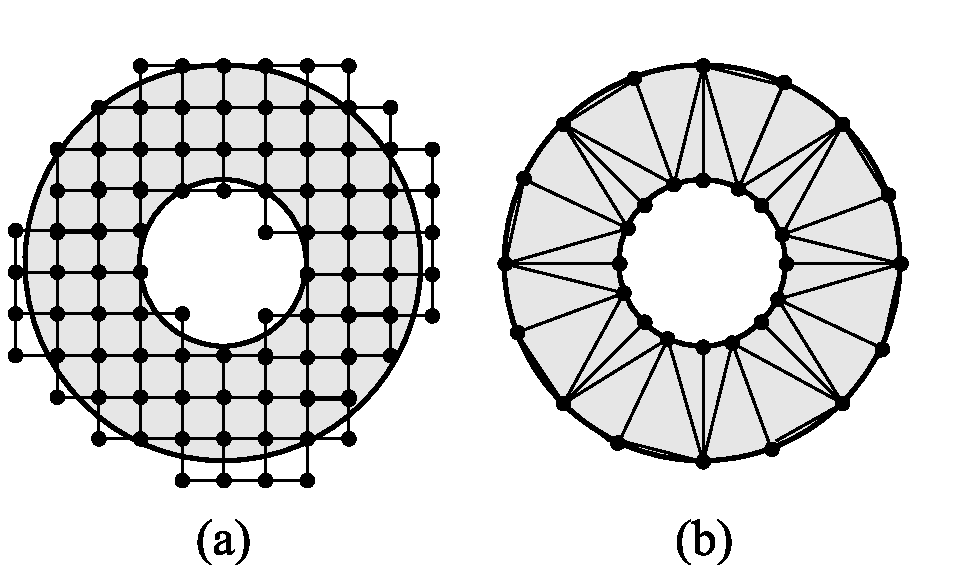
\includegraphics[scale=0.5]{figuras/fdm_fem.pdf}
	\caption{Método das diferenças Finitas e método dos Elementos Finitos}
	\label{fig:mdfFem}
\end{figure}

\subsection{Método dos Elementos Finitos}

O FEM surgiu originalmente como uma técnica de análise de deslocamentos e elasticidade de estruturas mecânicas, mas em seguida foi estendido para solucionar problemas de outros campos da física e da engenharia \cite{jin, desai, zien}.

As primeiras formulações do FEM são conhecidas como \textit{abordagem direta} ou \textit{formulação física}, que embora forneça a interpretação intuitiva do método, é util apenas para a resolução de problemas relativamente simples \cite{huebner, desai, zien}. O uso do princípio do trabalho virtual, para a determinação de forças na abordagem direta, levou à generalização do FEM, por meio da estratégia de minimização do funcional de energia. Esta técnica mais genérica  ficou conhecida como \textit{formulação variacional} \cite{desai, zien, jin} e tem como principal representante o método de Rayleigh-Ritz. Uma terceira abordagem, conhecida como \textit{Método dos Resíduos Ponderados} ou \textit{formulação generalizada} \cite{zien, huebner} é tradicionalmente utilizada e é ainda mais genérica que o princípio variacional, pois resolve diretamente as equações diferenciais do modelo, sem necessitar da existência de um funcional de energia \cite{desai}, ou ainda, sem exigir que o sistema seja positivo-definido. Neste trabalho será adotado o método dos resíduos ponderados, mais especificamente, o método de Galerkin.


\subsection{Método dos Resíduos Ponderados}
\label{sec:proc}

De acordo com \citeonline{jin}, a aplicação do FEM pode ser feita a partir de $4$ passos básicos: discretização do domínio, seleção das funções de interpolação, formulação do sistema de equações e solução do sistema de equações. Os três primeiros passos são descritos nos tópicos a seguir e o último na subseção \hyperref[sec:CG]{seguinte}.


\subsubsection*{Discretização do Domínio} 
A discretização do domínio consiste na transformação do contínuo $\Omega$ em uma malha de elementos finitos (discretos). Cada elemento $\Omega_e$ dessa malha representa um subdomínio de $\Omega$.  
Nesta etapa são definidas a forma, a quantidade e o tamanho dos elementos, de forma que a representação em malha seja a mais próxima possível do objeto em análise \cite{desai}.

Conforme pode ser visto na figura \ref{fig:numeracao}, cada elemento é identificado na malha a partir de um número que lhe é atribuído. Os vértices (ou nós) de cada elemento também são numerados. Cada nó possui dois valores vinculados a ele, um atuando como identificador global (numeração do nó na malha) e o outro como identificador local (numeração dentro de um dado elemento). A numeração local é geralmente feita no sentido anti-horário, a fim de se obter um valor positivo no cálculo da área ou volume por meio do  determinante \cite{sadiku, jin}. 

Um fator que deve ser levado em consideração é o balanceamento entre o refinamento da malha e o esforço computacional necessário \cite{desai}. Como o valor da solução é aproximado para cada elemento, o excesso de elementos pode causar a propagação do erro de aproximação, levando a resultados indesejáveis.


\begin{figure}[!htb]
	\centering
	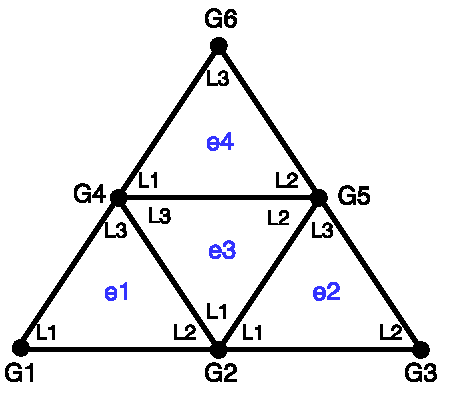
\includegraphics[scale=1.2]{figuras/id.pdf}
	\caption{Identificadores de elementos e nós}
	\label{fig:numeracao}
\end{figure}

\subsubsection*{Seleção das funções de interpolação}
\label{sec:interp}
O passo seguinte é a escolha das funções de interpolação (ou função de base ou de forma) \cite{huebner} que fornece uma aproximação da equação original dentro de cada subdomínio \cite{jin}. 
A função interpoladora escolhida geralmente é um polinômio, e isso ocorre por dois motivos a priori \cite{desai}:

\begin{itemize}  
	\item Facilidade de manipulação matemática, principalmente derivação e integração;
	\item Aproximação satisfatória quando truncado em uma ordem qualquer.
\end{itemize}

Na prática são escolhidos polinômios de primeira ou segunda ordem, mas ordens superiores podem ser adotadas para reduzir o erro de aproximação, sobretudo em bordas com curvaturas, no entanto, ocorre também o aumento da carga computacional \cite{jin}.

Seja a função $\phi$ desconhecida, da qual se deseja obter uma aproximação. A nível elementar, a função $\tilde{\phi^e}$ aproxima $\phi$ dentro do domínio do elemento $e$. Considerando um subdomínio bidimensional triangular a aproximação linear para o elemento $e$ pode ser feita como na equação \ref{eq:interp}. De acordo com esta aproximação, o valor em um dado nó $i$ pode ser obtido pela equação \ref{eq:interpNo}.

\begin{equation}
\label{eq:interp}
\tilde{\phi^e} = a^e + b^e x^e + c^e y^e
\end{equation}

\begin{equation}
\label{eq:interpNo}
\tilde{\phi^e_i} = a^e + b^e x^e_i + c^e y^e_i
\end{equation}

Após a resolução do sistema que contém as equações de todos os nós do elemento $e$, a fim de se obter os valores dos coeficientes $a$, $b$ e $c$ da aproximação, é obtida uma função de interpolação $N$ para os valores de $\phi$ no domínio de $e$. Conforme mostra a equação \ref{eq:interpol}, os valores $\phi^e$ em um ponto $(x,y)$ de $e$ podem ser aproximados a partir dos valores nodais $\phi^e_j$.

\begin{equation}
\label{eq:interpol}
\tilde{\phi^e} = \sum_{j=1}^{n}{N_j^e (x, y) \phi_j^e} = 
\{N^e\}^T \{\phi^e\}
\end{equation}

As funções $N_i^e$ obtidas interpolam os valores no interior do domínio e preservam os valores nodais $\tilde{\phi^e_1}$, $\tilde{\phi^e_2}$ e $\tilde{\phi^e_3}$. Para que isso ocorra, essas funções devem se comportar como o delta de Kronecker, como mostra a equação \ref{eq:kron} a seguir.

\begin{equation}
\label{eq:kron}
N_i^e(x^e_j, y^e_j) = \delta_{ij} = \begin{cases}
1, \ i = j\\
0, \ i \neq j
\end{cases}
\end{equation}

As funções de interpolação mais comuns pertencem às famílias de funções Lagrange e Serendipity \cite{zien, volakis}.

\subsubsection*{Formulação do sistema de equações}
Na abordagem variacional destaca-se o método de Ritz, ou Rayleigh-Ritz, o qual tem por objetivo, minimizar o funcional variacional, ou funcional de energia, do problema aproximado \cite{volakis}. Embora tal abordagem tenha sido historicamente utilizada e possua fundamentação física e matemática, sua adoção, em muitos casos, é mais complicada em relação ao Método dos Resíduos Ponderados, pois demanda a formulação variacional do problema. Desta forma, se um problema é dado por um modelo diferencial, é necessário se obter a partir deste modelo a forma variacional equivalente, para só então se aplicar o método para a obtenção do sistema de equações. No eletromagnetismo, a formulação variacional das equações de Maxwell não é bem estabelecida \cite{jin}.

Para problemas que apresentam explicitamente condições de Dirichlet no contorno e cujo operador $\mathcal{L}$ é linear e auto-adjunto, é possível se obter imediatamente o funcional de energia correspondente \cite{zien}, no entanto, como mostra \cite[p. 29]{volakis}, para este tipo de operador a mesma integral da formulação variacional é obtida pelo método de Galerkin.


Seja a equação \ref{eq:operador}, uma equação de um PVC na qual $\mathcal{L}$ é um operador diferencial, $f$ é uma função de excitação conhecida e $\phi$ é a solução procurada.

\begin{equation}
\label{eq:operador}
\mathcal{L} \phi = f
\end{equation}

Se substituirmos a solução exata pela sua aproximação apresentada na equação \ref{eq:interpol}, um resíduo $r$ surge, como pode ser visto na equação \ref{eq:residuos}, em decorrencia dos erros de aproximação.

\begin{equation}
\label{eq:residuos}
r = \mathcal{L} \tilde{\phi} - f \neq 0
\end{equation}

Embora o resíduo em cada elemento seja diferente de zero em sua maioria, deseja-se que o resíduo total seja igual a zero. Para que isso seja possível, uma função de poderação $w_i$ é introduzida para cada subdomínio $e$. Desta forma na média dos $M$ subdomínios de $\Omega$ a condição residual é atendida \cite{volakis}.
As equações \ref{eq:res1} e \ref{eq:res2} correspondem ao sistema de resíduos ponderados. A ideia chave dessa abordagem é transformar o problema de valor de contorno em um sistema linear que forneça o valor aproximado. 

\begin{equation}
\label{eq:res1}
R_i^e = \int_{\Omega}{w_i^e r \ d\Omega} = 0 \qquad i = 1,2,3.
\end{equation}

\begin{equation}
\label{eq:res2}
R_i^e = \int_{\Omega}{w_i^e [\mathcal{L} \tilde{\phi} - f] \ d\Omega} = 0  \qquad i = 1,2,3.
\end{equation}  


A escolha particular de $w_i^e = N^e_i$ configura o método de Galerkin, o qual, para um operador $\mathcal{L}$ auto adjunto a matriz do sistema é simétrica e equivalente à matriz gerada pelo método de Ritz. Após a substituição da equação \ref{eq:interpol} em \ref{eq:res2} obtem-se a equação \ref{eq:galerkin}, da qual são extraídas as matrizes elementares, como mostra a equação \ref{eq:sistema}.


\begin{equation}
\label{eq:galerkin}
R_i^e = \int_{\Omega}{N_i^e \mathcal{L} \left( \sum_{j=1}^{n}{N_j^e \phi_j^e} \right) } - \int_{\Omega}{N^e_i f \ d \Omega} = 0  \qquad i = 1,2,3.
\end{equation} 


\begin{equation}
\label{eq:sistema}
\sum_{j=1}^{n}\int_{\Omega}{N_i^e \mathcal{L} N_j^e  \phi_j^e  } = 0 \Rightarrow [K^e]\{\phi^e\} = \{b^e\} \qquad i = 1,2,3.
\end{equation}  

É importante colocar que o parâmetro $w_i$ deve ser um conjunto de funções integraveis e que respeitem as condições de contorno, ou seja, $w_i$ deve ser igual a zero nos nós de contorno do problema.
\cite{reddy}. Alguns casos especiais do método dos resíduos ponderados são obtidos a partir da escolha de $w_i$:

\begin{equation}
\label{eq:metPond}
\begin{tabular}{ l l }
Método de Petrov-Galerkin & $ w_i = \psi_i \neq \phi_i $ \\ 
Método de Galerkin & $ w_i = \phi_i $\\  
Método dos Mínimos quadrados & $ w_i = \frac{d}{dx} \left(a(x)\frac{d \phi_i}{dx}\right) $ \\ 
Método da colocação & $ \delta(x - x_i)  $ 
\end{tabular}
\end{equation}

Uma vez que as matrizes elementares foram obtidas é realizado o mapeamento dos identificadores locais para os identificadores globais. Este processo é conhecido como montagem da matriz global e é detalhado no apêndice \ref{ap:SED}. O sistema global é esparso e da ordem do número de nós da malha. As contribuições elementares (ou os coeficientes das matrizes de elementos) são agregados na matriz e as condições de contorno são aplicadas.

Neste trabalho são abordadas apenas as condições de contorno de Dirichlet. Essas condições, também conhecidas como essenciais, correspondem aos valores pre-estabelecidos da variável dependente. Dessa forma a definição do contorno consiste na substituição das incógnitas dos nós de contorno por seus respectivos valores. Assim, se um sistema de ordem $1000$ possui $200$ valores pré-fixados ele pode ser reduzido a ordem $800$. Um exemplo com os passos descritos nessa subseção é apresentado no apêndice \ref{sec:fem2d}.

\subsection{Método do Gradiente Conjugado}
\label{sec:CG}
O método do gradiente conjugado (CG) foi proposto por Hestenes e Stiefel em 1952 como um método direto para a solução de sistemas $n$ por $n$ positivos definidos (minimização do funcional de energia) \cite{burdenFaires}.
Embora sua concepção seja de um método exato que converge após $n$ iterações, sua aplicação tem sido feita como na forma de um método iterativo para se aproximar a solução de sistemas esparsos  \cite{Barrett1995}.
O método trabalha na busca da direção de mais decrescimento do funcional, ou seja, na direção contrária do vetor gradiente para problemas de minimização. Inicialmente é atribuído um ``chute'' para a solução, e à este chute é vinculado um certo resíduo, proporcional à distância entre o valor do chute e o valor da solução (mínimo do funcional). A cada iteração é calculada a correção da direção, a qual é tomada de tal forma que seja ortogonal às direções anteriores, impedindo que o método repita uma direção já percorrida. As direções ortogonais são obtidas por meio de sucessivas multiplicações da matriz do sistema pelo vetor direção. Dessa forma a aproximação da solução em cada iteração é encontrada em um subespaço de Krylov, como mostra a equação \ref{eq:krylov}. O pseudocódigo \ref{alg:kry} descreve as iterações do CG.

\begin{equation}
\label{eq:krylov}
K^m = span(d, Ad, A^2d, A^3d, ..., A^{m-1}d)
\end{equation}

\begin{algorithm}	
	\caption{\label{alg:kry}Algoritmo do Gradiente Conjugado} 
	\begin{algorithmic}[1]
		\State{$d_0 = r_0 = b - Ax_0$}		
		\For{j = 1,2...}
		\State{$\alpha = \frac{{r^i}^Tr^i}{{d^i}^TAd^i}$}
		\State{$x^{i+1} = x^i + \alpha d^i$}	
		\State{$r^{i+1} = r^i - \alpha d^i$}		
		\State{$\beta = \frac{{r^{i+1}}^Tr^{i+1}}{{r^i}^Tr^i}$}
		\State{$d^{i+1} = d^i - \beta d^i$}
		\If{$\frac{\parallel r^{i+1}\parallel}{\parallel b\parallel}$}
		\State{break}	
		\EndIf
		\EndFor
	\end{algorithmic}
\end{algorithm}



\chapter{Desenvolvimento}

O desenvolvimento deste trabalho está  dividido nas etapas de \textit{validação do problema} e \textit{aplicação das estratégias}. Na primeira são apresentados os recursos utilizados para modelar o problema e para definir as possíveis estratégias de solução. De posse das informações obtidas nesta etapa, são definidos na etapa seguinte os métodos e as estruturas de dados adotados em cada linguagem de programação e arquitetura de processamento.

\section{Materiais e métodos}
O ambiente de desenvolvimento \matlab foi adotado para a realização da etapa de validação do problema. A motivação dessa escolha se deu pela facilidade da manipulação de matrizes oferecida pelo ambiente e pela existência de ferramentas dedicadas à especificação de PVCs e à programação paralela.
A aplicação das estratégias propostas na etapa de validação nas linguagens e arquiteturas adotadas neste trabalho é feita pela adequação da sintaxe e do paradigma de programação da implementação realizada no \matlab. 

\subsection{Especificação da geometria}
O problema \textit{benchmark} utilizado neste trabalho é o exemplo $10.3$ do livro Análise de Circuitos de \citeonline{boylestad2011} e é ilustrado na figura \ref{fig:mesh}{(a)}. O capacitor é composto de duas placas quadradas paralelas com lado de $2$ polegadas, cuja distância entre elas é de $\frac{1}{32}$ polegadas. O problema informa que a diferença de potencial entre as placas é de $48V$, dessa forma foi assumido que uma das placas possui $48V$ e e que a outra está aterrada.

A fim de se realizar uma análise mais ampla do problema a distribuição do campo elétrico será calculada entre as placas mas também no espaço ao redor. Será considerada uma região quadrada de $16cm$ de lado como mostra o esquema na figura \ref{fig:mesh}{(b)}. Também foi considerado que a espessura de cada placa é a metade da largura da região entre elas, ou seja, $\frac{1}{64}$ polegadas.


A fim de se obter um parâmetro da corretude dos resultados obtidos neste trabalho, foi feita a simulação do problema na \textit{partial differential equation toolbox} do \matlab. Por meio dessa ferramenta é possível programaticamente e via interface gráfica definir a equação diferencial que rege o problema, a geometria, as condições de contorno, a malha inicial e seus refinamentos bem como a solução e exibição dos resultados do PVC. As figuras \ref{fig:mesh}{(c)} e \ref{fig:mesh}{(d)} mostram a geometria e a malha inicial modeladas com o auxílio da interface gráfica da \textit{pdetool}.

\subsection{Obtenção dos valores de referência}


\begin{figure}%
	\centering
	\subfloat[Perspectiva do capacitor de placas paralelas]{{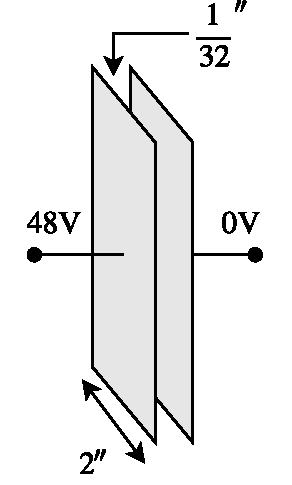
\includegraphics[scale=0.8]{figuras/placas.pdf} }}%
	\qquad	
	\subfloat[Esquema da região de análise]{{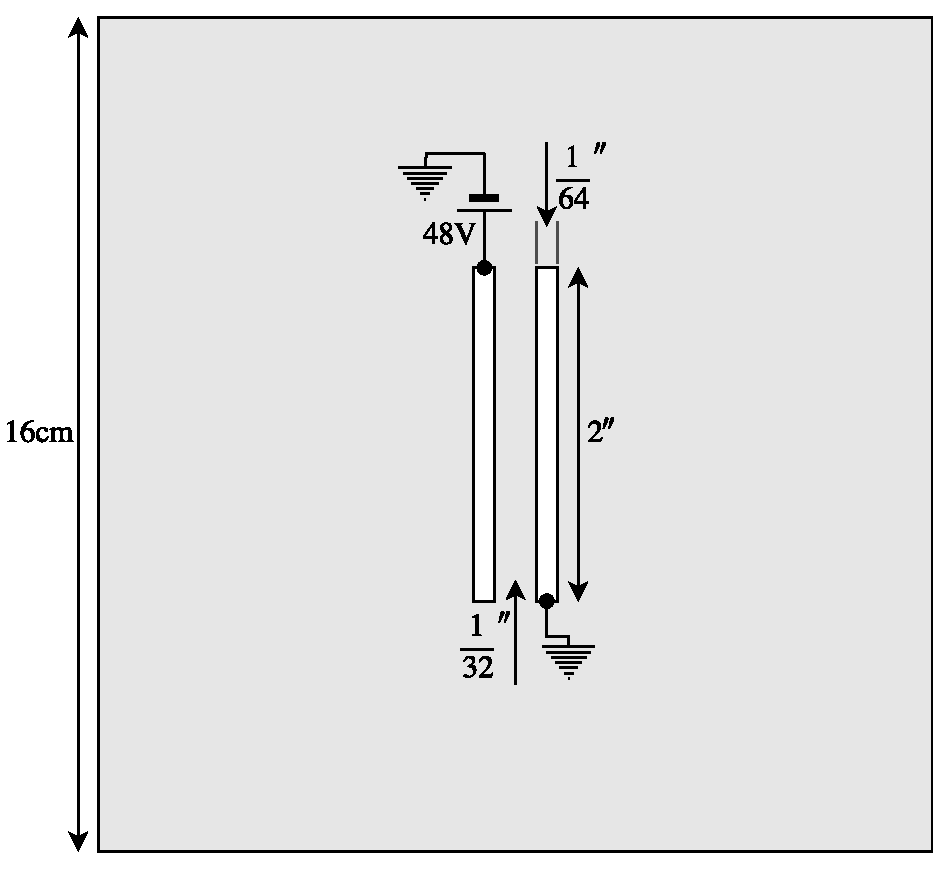
\includegraphics[scale=0.4]{figuras/espaco.pdf} }}%
	\qquad	
	\subfloat[Região de análise com malha]{{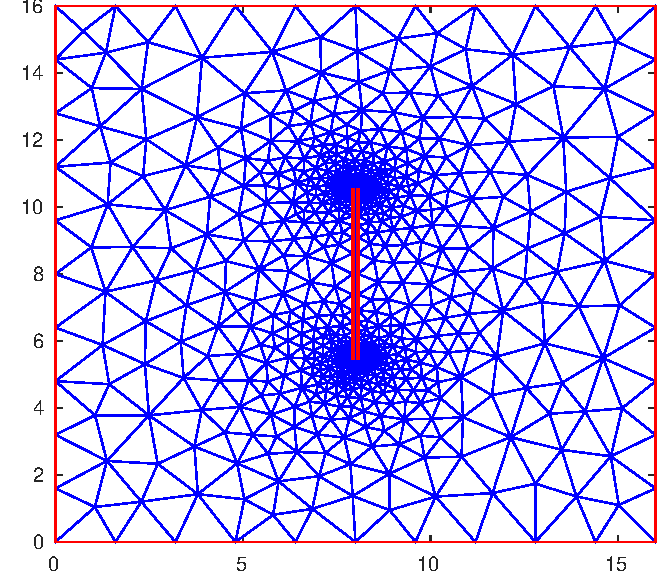
\includegraphics[scale=0.5]{figuras/mesh.pdf} }}%
	\qquad
	\subfloat[Zoom sobre as placas do capacitor]{{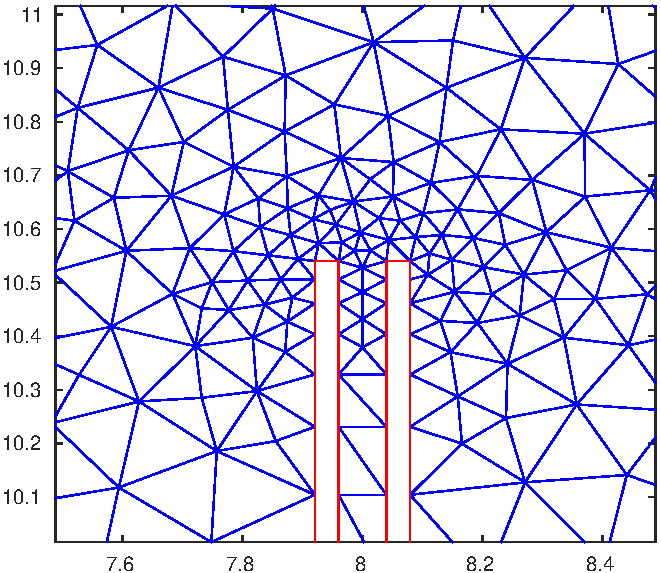
\includegraphics[scale=0.5]{figuras/meshzoom.pdf} }}%
	\caption{Geometria do capacitor de placas paralelas}%
	\label{fig:mesh}%
\end{figure}

Definidas a geometria e a malha, foram feitas as atribuições das condições de contorno de Dirichlet nas $4$ bordas da seção de cada placa. À placa da esquerda foram atribuídos $48V$ e $0V$ para a placa da direita. Para se definir a EDP do problema é necessário atribuir valores aos coeficientes da fórmula geral de EDPs elípticas, mostrada na equação \ref{eq:geral}.



\begin{equation}
\label{eq:geral}
- \bigtriangledown\cdot(c\bigtriangledown(u)) + au = f
\end{equation} 

Na equação de Laplace, que modela a distribuição do potencial elétrico, apenas o coeficiente $c$ é diferente de zero. A constante $c$ corresponde à permissividade no vácuo na equação de Poisson, mas como a densidade volumétrica de carga representada por $f$  e o auto valor $a$ são iguais a zero na equação de Laplace, $c$ passa a valer $1$. Estabelecidos os valores das constantes a solução do problema pode ser obtida, como mostram as figuras \ref{fig:solPde}{(a)} e \ref{fig:solPde}{(b)}.

\begin{figure}%
	\centering	
	\subfloat[Distribuição do potencial em Volts e fluxo do campo elétrico em Volts/centímetro (vetores normalizados)]{{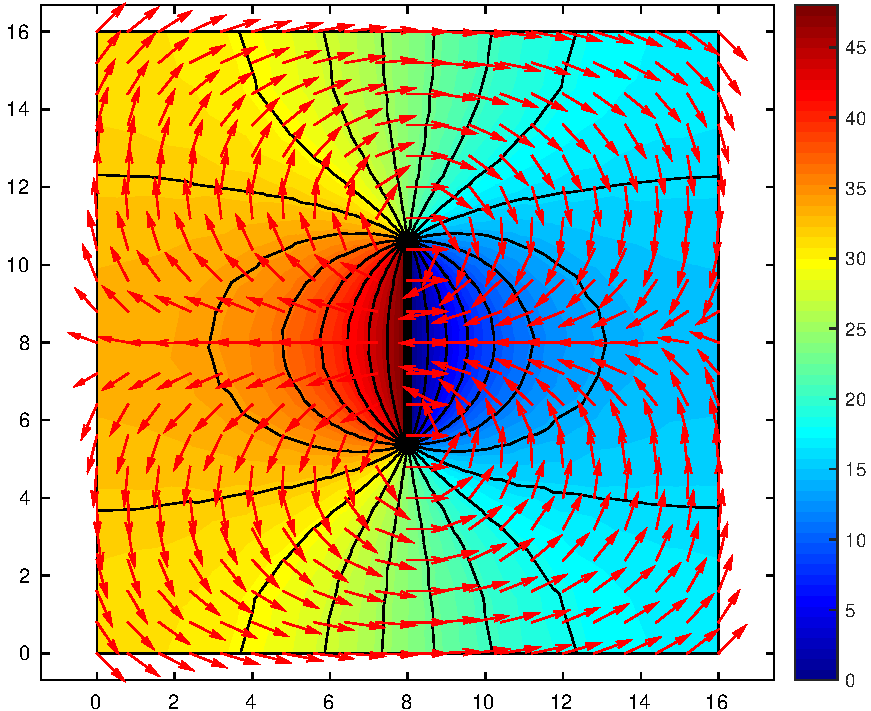
\includegraphics[scale=0.4]{figuras/potcampo.pdf} }}%
	\qquad
	\subfloat[Distribuição do potencial entre as placas]{{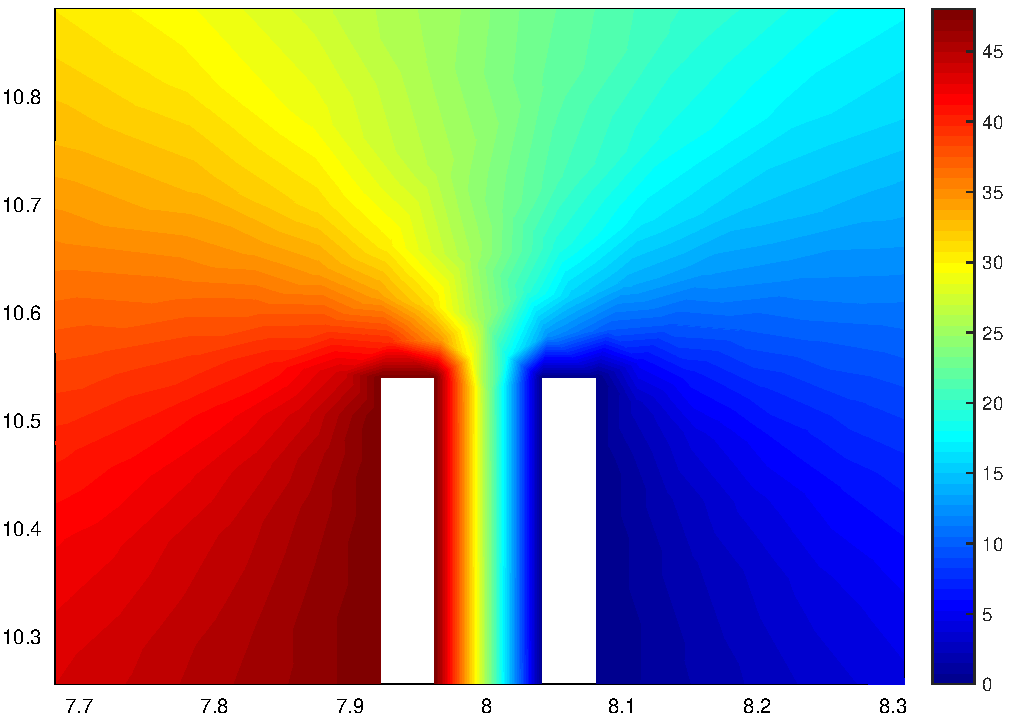
\includegraphics[scale=0.4]{figuras/potzoom.pdf} }}%
	\qquad
	\subfloat[Pontos de referência do potencial elétrico]{{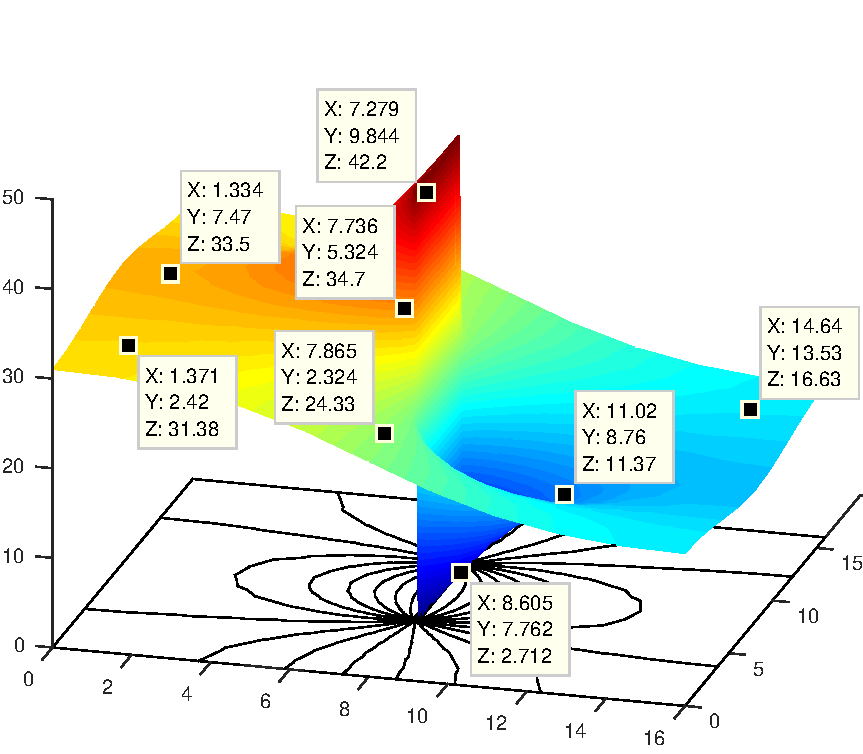
\includegraphics[scale=0.45]{figuras/valpot2.pdf} }}%
	\qquad
	\subfloat[Pontos de referência do campo elétrico]{{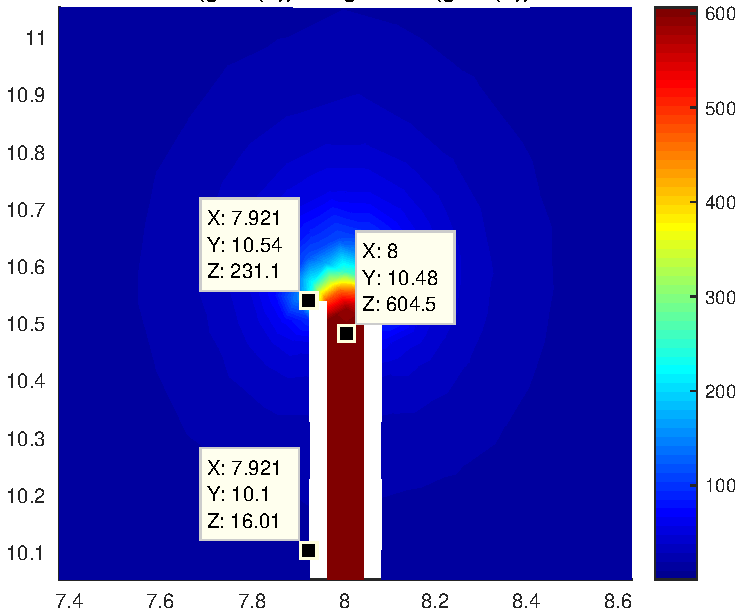
\includegraphics[scale=0.5]{figuras/valCampo.pdf} }}%
	\caption{Solução do PVC com a \textit{pdetool}}%
	\label{fig:solPde}%
\end{figure}

De posse da solução da \textit{pdetool}, foram tomados $8$ pontos de referência da distribuição do potencial e $3$ pontos de referência do campo elétrico. A localização e os valores destes pontos são apresentados na figuras \ref{fig:solPde}{(c)} e \ref{fig:solPde}{(d)}.

\subsection{Implementação do FEM}
Após a simulação e obtenção dos valores de referência foi realizada a implementação do método dos elementos finitos em duas dimensões, conforme o apresentado na seção \ref{sec:fem2d} do referencial teórico.
A fim de não tirar proveito das funções do \matlab de forma a manter a generalidade da solução implementada e a facilidade de transcrevê-la para outras linguagens, foram utilizadas nos algoritmos deste trabalho apenas as funções da \textit{PDE toolbox} relativas à geometria, geração da malha e exibição dos resultados. No pseudocódigo \ref{alg:FEM} as palavras destacadas em itálico são variáveis, as funções destacadas em negrito fazem parte do \matlab e as funções descritas nas linhas de $9$ a $12$ são detalhadas no exemplo da seção \ref{sec:fem2d}. A tabela \ref{tab:matlabFun} contém a descrição das funções utilizadas.

\begin{algorithm}	
	\caption{\label{alg:FEM}Pseudocódigo do FEM} 
	\begin{algorithmic}[1]
		\State{\textbf{load}($dadosGeometria$);}
		\State{\textbf{load}($coordReferencia$);}
		\State{\textbf{load}($dadosContorno$);}
		\State{$g$ = \textbf{decsg}($dadosGeometria$);}
		\State{$m$ = \textbf{createpde}(1);}
		\State{\textbf{geometryFromEdges}($m$,$g$);}
		\State{\textbf{generateMesh}($m$, 'Hmax',$valHmax$);}
		\State{($nos$,$tri$) = \textbf{meshToPet}($m.Mesh$);}
		\State{$C$ = geraMatElementares($nos$, $tri$);}
		\State{$G$ = geraMatGlobal($C$, $tri$);}
		\State{($A$, $b$) = atribuiContorno($G$, $dadosContorno$);}
		\State{$sol$ = resolveSistLinear($A$,$b$);}
		\State{\textbf{pdeplot}($m$,...);}
	\end{algorithmic}
\end{algorithm}


\begin{table}[!ht]   
	\centering
	\begin{tabular}{|l|p{10cm}|}  
		\hline
		\textbf{Função} 
		& \textbf{Descrição} 
		\\  
		\hline
		\textbf{load} 
		& Carrega para o \textit{workspace} as variáveis salvas nos arquivos \textit{.mat}. 
		\\
		\hline
		\textbf{decsg}  
		& Cria a geometria do problema por meio da associação de regiões primitivas. O espaço de análise do capacitor de placas paralelas, por exemplo é composto por $2$ retângulos e $1$ quadrado.
		\\
		\hline		
		\textbf{createpde} 
		& Instancia um modelo de PDE contendo $n$ equações.
		\\
		\hline		 
		\textbf{geometryFromEdges} 
		& Vincula a geometria originada da função $decsg$ ao modelo de PDE gerado por $createpde$.
		\\
		\hline		
		\textbf{generateMesh} 
		& Cria uma malha sobre a geometria do modelo de PDE. Parâmetros adicionais podem ser incluídos para modificar a qualidade malha ou a ordem dos elementos (ver \ref{sec:interp}). O parâmetro $Hmax$ determina o tamanho máximo das arestas dos elementos.
		\\
		\hline		 
		\textbf{meshToPet} 
		& Obtém as matrizes de pontos, arestas e triângulos, as quais serão utilizadas na geração das matrizes elementares e da matriz global.
		\\
		\hline	
		geraMatElementares
		& À partir dos dados da triangulação da malha, gera a matriz de cada elemento por meio das funções de aproximação e interpolação.
		\\
		\hline
		geraMatGlobal
		& Realiza a agregação ou o mapeamento das matrizes elementares no sistema global. A matriz resultante é esparsa e sua ordem corresponde ao número de nós da malha.
		\\
		\hline
		atribuiContorno  
		& Atribui os $m$ valores de contorno pré-estabelecidos e com isso realiza a redução dos sistema em $m$ ordens, fazendo com que deixe de ser homogêneo.
		\\
		\hline
		resolveSistLinear
		& Consiste na aplicação de métodos numéricos para a solução eficiente de sistemas lineares esparsos.
		\\
		\hline		 
		\textbf{pdePlot}  
		& Função utilizada para a exibição da malha e dos resultados. Conforme os parâmetros adicionais, são plotados gráficos tridimensionais, campos vetoriais e linhas de campo.
		\\
		\hline	
	\end{tabular}
	\caption{Descrição das funções utilizadas no algoritmo do FEM}
	\label{tab:matlabFun}
\end{table}
 


A função $resolveSistLinear$ é o ponto central deste trabalho, uma vez que a análise é feita sobre o desempenho das implementações na solução do sistema de equações originado do FEM. Foram utilizados $2$ \textit{solvers} a fim de se verificar a performance e a gestão de memória. O primeiro deles é o \textit{solver} ``$\setminus$'' do \matlab e o segundo é a implementação do método do gradiente conjugado proposta por \citeonline{Barrett1995}. O CG como explicitado no referencial teórico, é um método iterativo não estacionário do subespaço de Krylov. Como coloca \citeonline{Wathen1989}, o uso de métodos iterativos se tornou competitivo à medida em que os sistemas de equações se tornavam maiores. A técnica EBE foi proposta por \citeonline{Hughes1983} como como sendo um precondicionador para o CG de forma a possibilitar que as computações com matrizes sejam realizadas no nível elementar \cite{Kiss2012} de forma a possibilitar a vetorização (ou paralelização) e a economia de memória.

A motivação da escolha do \textit{solver} do \matlab (``$\setminus$'' ou $mldivide$) está no fato de ele utilizar diferentes algoritmos dependendo da estrutura da matriz de coeficientes, tais como simetria e esparsidade \cite{matMldivide}. Especificamente para o problema deste trabalho, cuja matriz é Hermitiana (auto-adjunta) e positiva definida, o \textit{solver} adota a fatoração de Cholesky ou a LDL.

A motivação para a escolha do CG implementado por \citeonline{Barrett1995} está no fato de que seu material é citado em diferentes trabalhos da revisão bibliográfica, como em \citeonline{Kiss2012, Dolwithayakul2012, Yang2016}. Além de um completo \textit{survey} de métodos numéricos para a solução de sistemas lineares, os autores disponibilizam as implementações na linguagem do \matlab e em C++. O pseudocódigo do CG precondicionado com a matriz $M$ é apresentado em \ref{alg:CG} e a descrição de cada etapa é apresentada na seção \ref{sec:CG} da fundamentação teórica.

\begin{algorithm}	
	\caption{\label{alg:CG}Pseudocódigo do CG} 
	\begin{algorithmic}[1]
		\State{$x_{0}$ = $\{0\}$}
		\State{$r_{0}$ = $b - Ax_0$}
		\For{i = 1,2...}
			\State{$z_{i-1}$ = resolve($M$, $r_{i-1}$)}
			\State{$\rho_{i-1}$ = ${r_{i-1}}^{T}z_{i-1}$}
			\If{i = 1}
				\State{$p_1$ = $z_0$}
				\Else
				\State{$\beta_{i-1}$ = $\rho_{i-1}$ / $\rho_{i-2}$}
				\State{$p_{i}$ = $z_{i-1}$ + $\beta_{i-1}p_{i-1}$}
			\EndIf	
			\State{$q_i$ = $Ap_i$}
			\State{$\alpha_{i}$ = $\rho_{i-1}$ / ${p_{i}}^Tq_i$}
			\State{$x_{i}$ = $x_{i-1}$ + $\alpha_{i}p_{i}$}
			\State{$r_{i}$ = $r_{i-1}$ - $\alpha_{i}q_{i}$}
			\If{converge($r$,$tol$)}
				\State{break}
			\EndIf
		\EndFor
	\end{algorithmic}
\end{algorithm}





\subsection{Implementação do EBE-FEM}
A implementação do EBE-FEM consiste basicamente em antecipar a solução do sistema de equações, passando da montagem das matrizes elementares diretamente para a atribuição das condições de contorno e solução do sistema, sem que seja necessária a montagem da matriz de coeficientes global. Para realizar esta mudança de rota na solução do problema é necessário modificar tanto o algoritmo quanto a estrutura de dados utilizados.

A adaptação do bloco referente à atribuição das condições de contorno (linha $11$ do algoritmo \ref{alg:FEM}) é baseada na abordagem proposta por  \citeonline{Xu2005} a qual consiste na criação de vetores \textit{rhs} (\textit{right hand side}) elementares. Ao invés de se atribuir os valores de contorno às células do vetor \textit{rhs} global que correspondem à cada nó da malha, a atribuição é feita no nível elementar. Por exemplo, se um nó compartilhado por $2$ elementos possui valor de contorno igual a $10$, a atribuição é feita como uma média no vetor \textit{rhs} de cada um dos $2$ elementos. Assim sendo, cada vetor recebe o valor de contorno igual a $5$. A figura \ref{fig:contornoEBE} contém o esquema que ilustra este exemplo. \citeonline{Yan2017} e \citeonline{Wu2015} propõe uma abordagem parecida baseada não no número de conexões do nó, mas na média ponderada do valor de contorno original pelos coeficientes de cada elemento que contém o nó. 

\begin{figure}[!htb]
	\centering
	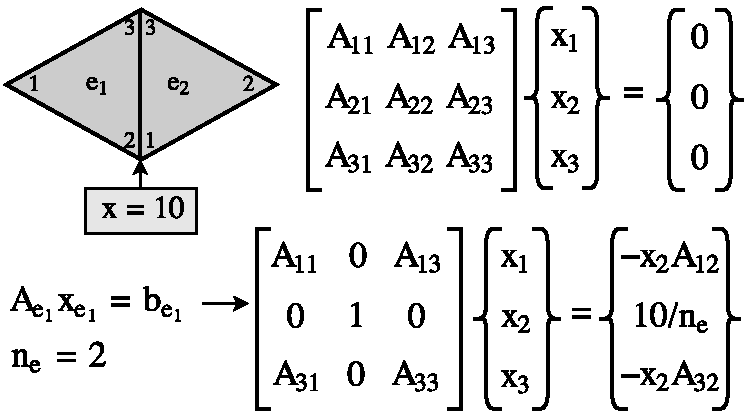
\includegraphics[scale=0.8]{figuras/contorno.pdf}
	\caption{Esquema da aplicação das condições de contorno de um elemento}
	\label{fig:contornoEBE}
\end{figure}

De posse das matrizes e vetores elementares com as condições de contorno atribuídas, é feita a adaptação no algoritmo do  CG a fim de que os cálculos envolvendo matrizes sejam feitos elemento a elemento. As operações entre vetores e escalares são mantidas no nível global, visto que não requerem tanto esforço computacional como as operações matriciais.  As adaptações consistem basicamente em percorrer os $N$ elementos, realizando os cálculos pertinentes e em seguida, armazenar nos vetores globais os resultados gerados para cada nó do elemento. As linhas $4$ e $12$ do algoritmo \ref{alg:CG} possuem operações matriciais e são modificadas conforme apresentado nos pseudocódigos \ref{alg:ebeCG1} e \ref{alg:ebeCG2}. Além disso, o resíduo inicial da linha $2$ do \ref{alg:CG} é igual a $b$ , dado que o chute $x_0$ vale zero para todos os nós. Como os valores de $b$ foram atribuídos pelas condições de contorno em nível elementar, é necessário realizar a montagem do vetor $b$ global para a determinação do resíduo inicial aconteça. Este processo de montagem é apresentado no pseudocódigo \ref{alg:ebeCG3}.

\begin{algorithm}	
	\caption{\label{alg:ebeCG1}Adaptação da declaração $z_{i-1}$ = resolve($M$, $r_{i-1}$)} 
	\begin{algorithmic}[1]
		\State{$z$ = $\{0\}$}		
		\For{j = 1,2...$|tri|$}
		\State{$map = tri(j)$}
		\State{$M_e = precond(A_e(j))$}
		\State{$z(map) = z(map) + M_er(map)$}
		\EndFor
	\end{algorithmic}
\end{algorithm}

\begin{algorithm}	
	\caption{\label{alg:ebeCG2}Adaptação da declaração $q_i$ = $Ap_i$} 
	\begin{algorithmic}[1]
		\State{$q$ = $\{0\}$}		
		\For{j = 1,2...$|tri|$}
		\State{$map = tri(j)$}
		\State{$q(map) = q(map) + A_e(j)q(map)$}
		\EndFor
	\end{algorithmic}
\end{algorithm}

\begin{algorithm}	
	\caption{\label{alg:ebeCG3}Adaptação da declaração $r_{0}$ = $b - Ax_{0}$} 
	\begin{algorithmic}[1]
		\State{$b$ = $\{0\}$}		
		\For{j = 1,2...$|tri|$}
		\State{$map = tri(j)$}
		\State{$b(map) = b(map) + b_e(j)$}
		\EndFor
		\State{$r_{0}$ = $b$}
	\end{algorithmic}
\end{algorithm}

\subsection{Coloração da malha}
Proposta por \citeonline{Wathen1989} e implementada por \citeonline{Kiss2012} a coloração da malha possibilita que os trechos do CG descritos nos algoritmos \ref{alg:ebeCG1}, \ref{alg:ebeCG2} e \ref{alg:ebeCG3} sejam paralelizados. A coloração assim como o processo de exclusão mútua são estratégias adotadas para evitar condições de corrida. Condição de corrida é o estado inconsistente dos dados causado por transações não atômicas. Desta forma, se por exemplo, dois processos ou \textit{threads} alteram ao mesmo tempo um dado em memória compartilhada, não se pode prever o valor final do dado, mas sabe-se que será inconsistente. A coloração deve acontecer de tal forma que elementos que compartilhem um mesmo nó possuam cores distintas. Uma característica desejável num algoritmo otimizado é que haja uma distribuição equalizada na quantidade elementos de cada cor, ao invés de uma quantidade mínima de cores. Por exemplo, numa malha de $1000$ elementos é preferível se utilizar $20$ cores com $50$ elementos de cada cor, ao invés de $6$ cores com uma distribuição desequilibrada de elementos, como por exemplo $\{500 \ 50 \ 200 \ 150 \ 10 \ 90\}$. Contudo, como o objetivo da etapa de \textit{validação do problema} não é obter resultados ótimos, foi adotada uma heurística gulosa sem balanceamento de cores, mas que apenas prioriza a aplicação das cores menos utilizadas. A figura \ref{fig:color} mostra um zoom na coloração da malha no topo entre as duas placas.

\begin{figure}[!htb]
	\centering
	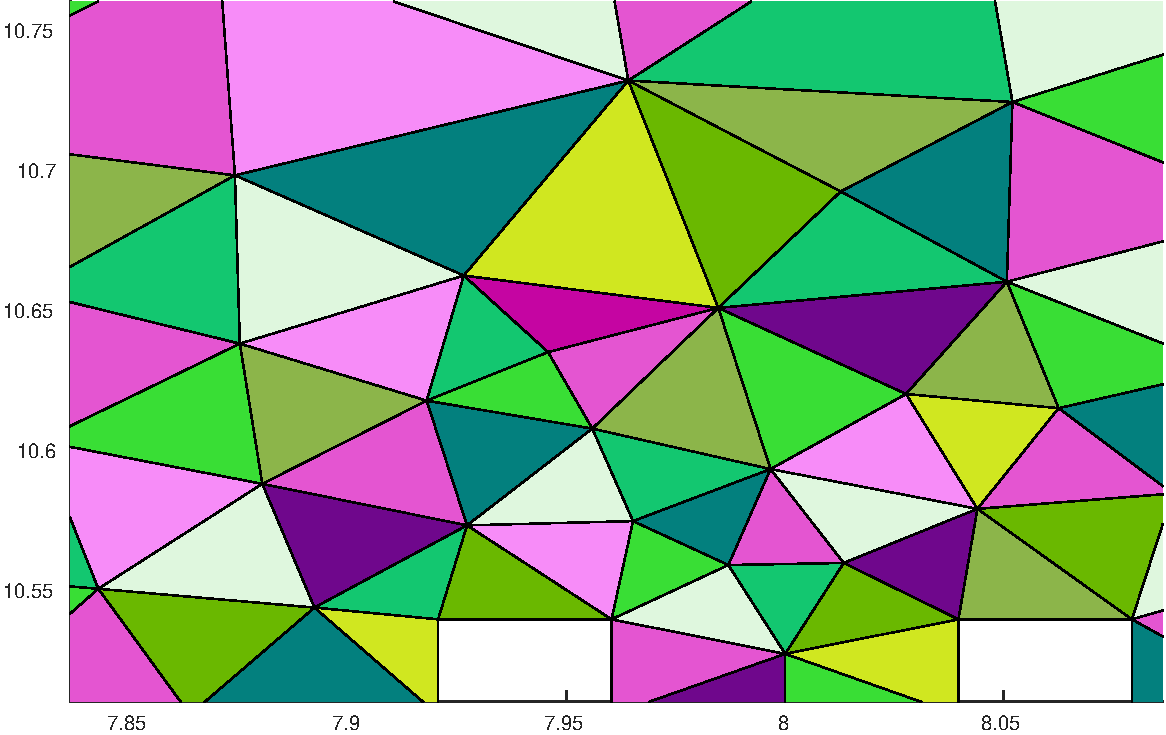
\includegraphics[scale=0.5]{figuras/color.pdf}
	\caption{Exemplo de coloração da malha}
	\label{fig:color}
\end{figure}

Uma vez realizada a coloração, o processamento pode ocorrer de tal forma que elementos da mesma cor seja executados simultaneamente e elementos de cores distintas sequencialmente. Como elementos de uma determinada cor não possuem vértices em comum, não há a possibilidade de acontecer condição de corrida durante o acesso às variáveis globais $z$ e  $r$ do algoritmo \ref{alg:ebeCorCG1} e $q$ e $d$ dos algoritmos \ref{alg:ebeCorCG2} e \ref{alg:ebeCorCG3} respectivamente. A estrutura de dados $cores$ contém os dados da localização do elemento na malha.

\begin{algorithm}	
	\caption{\label{alg:ebeCorCG1}Aplicação da coloração no algoritmo \ref{alg:ebeCG1}} 
	\begin{algorithmic}[1]
		\State{$z$ = $\{0\}$}
		\For{c = 1,2...$|cores|$}	
		\State{$triCor = cores(c)$}	
		\For{j = 1,2...$|triCor|$}
		\State{$idG = triCor(j)$}
		\State{$map = tri(idG)$}
		\State{$M_e = precond(A_e(idG))$}
		\State{$z(map) = z(map) + M_er(map)$}
		\EndFor
		\EndFor
	\end{algorithmic}
\end{algorithm}

\begin{algorithm}	
	\caption{\label{alg:ebeCorCG2}Aplicação da coloração no algoritmo \ref{alg:ebeCG2}} 
	\begin{algorithmic}[1]
		\State{$q$ = $\{0\}$}
		\For{c = 1,2...$|cores|$}	
		\State{$triCor = cores(c)$}					
		\For{j = 1,2...$|triCor|$}
		\State{$idG = triCor(j)$}
		\State{$map = tri(id)$}
		\State{$q(map) = q(map) + A_e(idG)q(map)$}
		\EndFor
		\EndFor
	\end{algorithmic}
\end{algorithm}

\begin{algorithm}	
	\caption{\label{alg:ebeCorCG3}Aplicação da coloração no algoritmo \ref{alg:ebeCG3}} 
	\begin{algorithmic}[1]
		\State{$b$ = $\{0\}$}
		\For{c = 1,2...$|cores|$}	
		\State{$triCor = cores(c)$}					
		\For{j = 1,2...$|triCor|$}
		\State{$idG = triCor(j)$}
		\State{$map = tri(idG)$}
		\State{$b(map) = b(map) + b_e(idG)$}
		\EndFor
		\EndFor
		\State{$r_{0}$ = $b$}
	\end{algorithmic}
\end{algorithm}

\subsection{Paralelização do algoritmo}
A fim de manter a conformidade com o ambiente de desenvolvimento optou-se por utilizar a \textit{parallel Computing toolbox} do \matlab. Esta ferramenta possibilita a implementação para plataformas \textit{multicore}, GPUs, \textit{clusters}, \textit{grids} e \textit{cloud}. De acordo com a documentação do \matlab \cite{matMulticore}, funções de álgebra linear como $fft$, $mldivide$, $eig$, $svd$, e $sort$
são \textit{multithread} desde a versão R2018a. No entanto, é possível melhorar a performance de funções customizadas por meio da \textit{parallel toolbox}.

A fim de garantir a robustez do código paralelizado, o \matlab disponibiliza a programação em múltiplos \textit{workers} ao invés de \textit{threads}. Cada \textit{worker} é um processo que trabalha em função do processo principal (\textit{client}) que o originou. Desta forma, as tarefas são divididas entre os \textit{workers} e coordenadas pelo \textit{client}, num modelo mestre-escravo. A fim de evitar condições de corrida e o \textit{overhead} de comunicação entre os processos, a ferramenta trabalha por meio de distribuição e troca de mensagens (MPI) ao invés do compartilhamento de memória. Assim sendo, os dados são copiados para cada \textit{worker} e ao final do processamento, agregados novamente no \textit{client}. A tabela \ref{tab:partool} contém a descrição das funções utilizadas da \textit{parallel toolbox}.


\begin{table}[!ht]   
	\centering
	\begin{tabular}{|l|p{10cm}|}  
		\hline
		\textbf{Função} 
		& \textbf{Descrição} 
		\\  
		\hline
		\textbf{gcp} 
		& \textit{Get current parallel pool} retorna as informações sobre os \textit{workers} ativos.
		\\
		\hline
		\textbf{parpool}  
		& Cria uma nova \textit{parallel pool}, ou seja, um conjunto de \textit{workers} e os demais processos necessários para o funcionamento da \textit{toolbox}.
		\\
		\hline		
		\textbf{parfor} 
		& Executa as iterações de um \textit{loop} em \textit{workers}. Para que isso seja possível as iterações devem ser independentes entre si e as estruturas de dados (coleções) utilizadas devem ter a característica de serem ``fatiadas''.  Por exemplo, uma matriz bidimensional pode ser fatiada de $2$ formas, pelas linhas ou pelas colunas.
		\\
		\hline		 
		\textbf{spmd} 
		& A função \textit{single program, multiple data} executando o mesmo código em diferentes \textit{workers}. Diferente do \textit{parfor}, os dados não precisam necessariamente estar particionados, visto que o \textit{spmd} permite a comunicação entre os \textit{workers}.
		\\
		\hline		
		\textbf{codistributed} 
		& Cria uma coleção que é distribuída entre os \textit{workers} e não copiada integralmente.
		\\
		\hline		 
		\textbf{getLocalPart} 
		& Obtém os dados de uma determinada partição de uma coleção distribuída.
		\\
		\hline	
		\textbf{codistributor}
		& Função que realiza a distribuição de uma coleção. Diferente da distribuição limitada que ocorre no \textit{parfor}, essa função possibilita que a distribuição seja feita de diferentes formas em uma coleção. 
		\\
		\hline
		\textbf{gather}
		& Função que realiza a agregação de uma coleção distribuída.
		\\
		\hline
		\textbf{drange}  
		& Executa um \textit{loop} entre as partições de uma coleção. Este bloco de código faz com que os \textit{workers} trabalhem simultaneamente em cada distribuição da coleção, mas impede a comunicação entre eles.
		\\
		\hline	
	\end{tabular}
	\caption{Descrição das funções utilizadas na paralelização do EbE-FEM}
	\label{tab:partool}
\end{table}

Para que a paralelização do código ocorra por meio das funções \textit{parfor} e \textit{spmd} é necessário que a estrutura de dados da coloração seja modificada, a fim de que possa ser ``fatiada'' e distribuída entre os \textit{workers}. Como pode ser visto nos algoritmos de \ref{alg:ebeCorCG1} a \ref{alg:ebeCorCG3}, as variáveis globais são indexadas pela variável $map$, que contém a lista dos identificadores de cada nó do elemento, como por exemplo $\{25 \ 12 \ 96\}$. Como estes índices não são contíguos, ocorre um erro durante a compilação do \textit{parfor} e o \textit{overhead} de comunicação no \textit{spmd}. Esta restrição do \matlab demanda uma nova adaptação da estrutura de dados e impede que a atribuição às variáveis globais seja feita de forma paralela.

A nova estrutura de dados gerada durante a coloração já retorna o vetor $b$ (ou $rhs$) completo, dessa forma, não há a necessidade do processo de montagem à partir dos vetores elementares, como descrito nos algoritmos \ref{alg:ebeCG3} e \ref{alg:ebeCorCG3}. Além dessa melhoria, o objeto retornado da coloração possui para cada cor, as matrizes elementares e o vetor $rhs$ referente aos elementos da cor. Em resumo, a nova abordagem retorna os próprios objetos que serão utilizados na paralelização ao invés do seu ``endereço'' na malha. Os pseudocódigos \ref{alg:ebeParCG1} e \ref{alg:ebeSpmdCG1} mostram a aplicação das funções \textit{parfor} e \textit{spmd} no algoritmo \ref{alg:ebeCorCG1}. A mesma adaptação é feita para o algoritmo \ref{alg:ebeCorCG2}.



\begin{algorithm}	
	\caption{\label{alg:ebeParCG1}Aplicação do \textit{parfor} no algoritmo \ref{alg:ebeCorCG1}} 
	\begin{algorithmic}[1]
		\For{c = 1,2...$|cores|$}
		\State{$matElCor = cores(c).matEl$}
		\State{$rhsCor = cores(c).rhs$}		
		\State{$R = reshape(r(rhsCor),3,[ \ ])$}
		\State{\textbf{PARFOR}}	
		\For{j = 1,2...$|cores(c)|$}
		\State{$M_e = precond(matElCor(j))$}
		\State{$Z = M_eR(j)$}
		\EndFor
		\State{\textbf{END PARFOR}}
		\State{$z(rhsCor) = z(rhsCor) + reshape(Z,1,[ \ ])$}
		\EndFor
	\end{algorithmic}
\end{algorithm}

\begin{algorithm}	
	\caption{\label{alg:ebeSpmdCG1}Aplicação do \textit{spmd} no algoritmo. \ref{alg:ebeCorCG1}} 
	\begin{algorithmic}[1]
		\For{c = 1,2...$|cores|$}
		\State{$matElCor = cores(c).matEl$}
		\State{$rhsCor = cores(c).rhs$}		
		\State{$R = reshape(r(rhsCor),3,[ \ ])$}
		\State{\textbf{SPMD}}
		\State{$codMat = codistributor(formaDistMat)$}
		\State{$MatDist=codistributed(matElCor,codMat)$}	
		\State{$codR = codistributor(formaDistR)$}
		\State{$RDist = codistributed(R,codR)$}

		\State{$MatPart = getLocalPart(MatDist)$}
		\State{$RPart = getLocalPart(RDist)$}
		\For{j = 1,2...$qtdWorkers$}
		\For{k = 1,2...$|cores(c)|$}
		\State{$M_e = precond(MatPart(j,k))$}
		\State{$Z = M_eRPart(j,k)$}
		\EndFor
		\EndFor
		\State{\textbf{END SPMD}}
		\State{$z(rhsCor) = z(rhsCor) + reshape(Z,1,[ \ ])$}
		\EndFor
	\end{algorithmic}
\end{algorithm}

Enquanto a paralelização por \textit{parfor} é feita elemento a elemento, a função \textit{spmd} distribui o processamento em $q$ partes, sendo $q$ a quantidade de \textit{workers}. Cada \textit{worker} executa sequencialmente a parcela do problema que lhe é atribuída. Conforme a recomendação da documentação, para se obter melhor desempenho, a quantidade de \textit{workers} deve ser a mesma de núcleos físicos do processador. Ao se utilizar o bloco $for-drange$ na linha $13$ ao invés do $for$ convencional, o comportamento do $spdm$ passa a ser equivalente ao do $parfor$.


\section{Resultados}
Os resultados deste trabalho estão divididos nas subseções \textit{resultados preliminares} e \textit{resultados aplicados}. Na primeira subseção são apresentados os resultados da modelagem com o \matlab e na subseção seguinte os resultados da aplicação do algoritmo desenvolvido nas linguagens C++, Scala, Erlang, CUDA e Harlan.

\subsection{Resultados preliminares}
O objetivo desta primeira etapa de atividades é validar o processo de paralelização do EbE-FEM na tentativa de antecipar as possíveis dificuldades que possam surgir na implementação do algoritmo nas linguages concorrentes e paralelas e nas arquiteturas multi e \textit{manycore}. 


\subsubsection*{\textit{Overview} da triangulação}
No início do desenvolvimento foram selecionados pontos de referência a fim de se estimar a precisão das aproximações, com base nos resultados da \text{pdetool} (figura \ref{fig:solPde}).
A \textit{pdetool} forneça a opção de refinamento da malha, que consiste na subdivisão dos triângulos já existentes, no entanto, a opção de refinamento programático disponibilizada pela \textit{toolbox} é dada pelo parâmetro \textit{Hmax} da função \textit{generateMesh} (algoritmo \ref{alg:FEM}). Enquanto o refinamento da \textit{pdetool} mantém os pontos da malha original, a alteração do \textit{Hmax} gera uma nova malha, fazendo com que os pontos de referência se percam. Embora essa abordagem possibilite o maior controle da quantidade de elementos, ela impossibilita a verificação da precisão do valor de um ponto após o refinamento. A figura \ref{fig:vizinha} destaca os nós da vizinhança de cada ponto de referência. Como não se pôde observar a precisão foi observado o valor médio próximo aos pontos de referência.  A tabela \ref{tab:hmax} apresenta a quantidade de elementos e nós gerados para cada valor de $Hmax$.


\begin{figure}%
	\centering	
	\subfloat[Refinamento com $Hmax = 0.6$]{{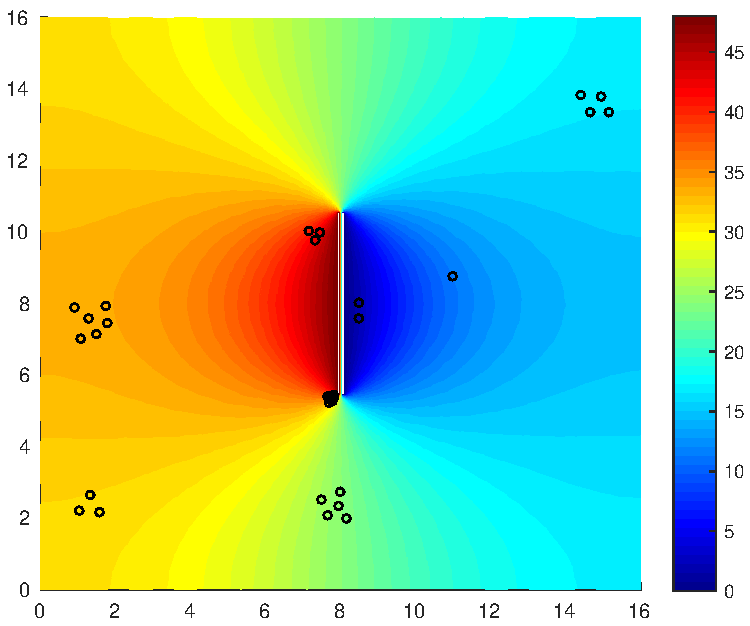
\includegraphics[scale=0.5]{figuras/viz0_6.pdf} }}%
	\qquad
	\subfloat[Refinamento com $Hmax = 0.2$]{{\includegraphics[scale=0.5]{figuras/viz0_2.pdf} }}%
	\caption{Vizinhança dos pontos de referência}%
	\label{fig:vizinha}%
\end{figure}

 \begin{table}
	\centering
	\begin{tabular}{|l|l|l|}  
		\hline
		\textbf{Hmax} & \textbf{Nós} & \textbf{Elementos} \\ 
		\hline
		$0.6$ & $1700$ & $3190$ \\
		\hline
		$0.5$ & $2196$ & $4162$ \\
		\hline
		$0.4$ & $3154$ & $6046$ \\
		\hline
		$0.3$ & $5287$ & $10244$ \\
		\hline
		$0.2$ & $11439$ & $22416$ \\       
		\hline
		$0.1$ & $44692$ & $88522$ \\       
		\hline
		$0.05$ & $176971$ & $352148$ \\       
		\hline				
	\end{tabular}
	\caption{Mapeamento dos identificadores locais do circuito da figura \ref{fig:malhaGenerica}}
	\label{tab:hmax}
\end{table}

\subsubsection*{\textit{Overview} das implementações}
Conforme apresentado no capítulo de materiais e métodos, foram desenvolvidas duas versões do algoritmo  do EbE-FEM, sendo a primeira adequada para sistemas de memória compartilhada e \textit{multithread} (algoritmos \ref{alg:ebeCorCG1} a \ref{alg:ebeCorCG3}) e a segunda para sistemas de memória distribuída (\ref{alg:ebeParCG1} e \ref{alg:ebeSpmdCG1}).
A primeira versão do algoritmo proposta por \citeonline{Kiss2012} apresenta coloração e é paralelizável, no entanto, devido às restrições dos blocos \textit{parfor} e \textit{spmd} da \textit{parallel computing toolbox} do \matlab foi possível testá-la apenas em sua sequencialmente.
A segunda implementação utiliza uma estrutura de dados distribuída e desacoplada para atender aos critérios de ``fatiamento'' e independência dos blocos \textit{parfor} e \textit{spmd}.

A tabela \ref{tab:seq} exiibe os resultados das execuções com o uso de \textit{solvers} sequenciais. as linhas indicadas com $x$ mostram as limitações do processo de montagem da matriz global devido ao uso excessivo de memória. A mensagem de erro retornada pelo \matlab é \textit{Requested 44692x44692 (14.9GB) array exceeds maximum array size preference}. A adoção do mecanismo de matrizes esparsas do \matlab no entanto possibilitou que o uso de memória e o percentual de CPU fossem reduzidos. Os \textit{solvers} de matrizes esparsas e o EbE apresentaram um uso equilibrado da CPU em relação ao \textit{mldivide} e \textit{CG} com matrizes \textit{full} que aumentaram o percentual do uso da CPU à medida que o número de elementos da malha aumentou. A figura \ref{fig:grafSeq} exibe a comparação do tempo de processamento e uso de memória dos \textit{solvers} mais competitivos para para os refinamentos $0.3$, $0.2$ e $0.1$.

\begin{figure}%
	\centering	
	\subfloat[Comparação do tempo de execução (s)]{{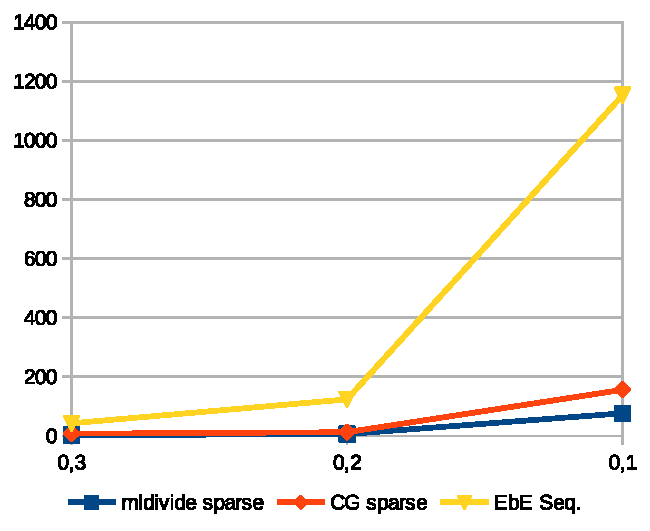
\includegraphics[scale=0.6]{figuras/grafSeqTempo.pdf} }}%
	\qquad
	\subfloat[Comparação do uso de memória (MiB)]{{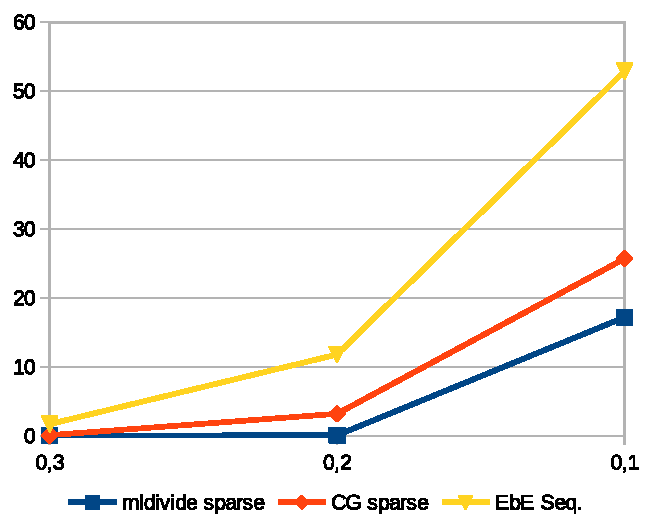
\includegraphics[scale=0.6]{figuras/grafSeqMemo.pdf} }}%
	\caption{Comparação do EbE com soluções sequenciais eficientes}%
	\label{fig:grafSeq}%
\end{figure}

\begin{table}[]
	\centering
	\begin{tabular}{|l|l|l|l|l|}
		\hline
		\textbf{Solver}                         & \textbf{Hmax} & \textbf{Tempo (s)} & \textbf{Memo (MiB)} & \textbf{\%CPU} \\ \hline
		\multirow{6}{*}{\textbf{mldivide}}        & 0.6           & 0.390717           & 22.1                & 8              \\ \cline{2-5} 
		& 0.5           & 0.524704           & 37                  & 24             \\ \cline{2-5} 
		& 0.4           & 0.911115           & 81.8                & 28             \\ \cline{2-5} 
		& 0.3           & 2.572255           & 215.2               & 29             \\ \cline{2-5} 
		& 0.2           & 21.337269          & 995                 & 50             \\ \cline{2-5} 
		& 0.1           & x                  & x                   & x              \\ \hline
		\multirow{3}{*}{\textbf{mldivide Sparse}} & 0.3           & 2.447401           & 0.05                & 25             \\ \cline{2-5} 
		& 0.2           & 6.158577           & 0.08                & 26             \\ \cline{2-5} 
		& 0.1           & 76.558448          & 17.2                & 29             \\ \hline
		\multirow{6}{*}{\textbf{CG}}            & 0.6           & 0.541897           & 32.9                & 19             \\ \cline{2-5} 
		& 0.5           & 0.789027           & 36.2                & 16             \\ \cline{2-5} 
		& 0.4           & 1.56392            & 71.3                & 27             \\ \cline{2-5} 
		& 0.3           & 4.562658           & 210.7               & 51             \\ \cline{2-5} 
		& 0.2           & 27.876141          & 1006.3              & 55             \\ \cline{2-5} 
		& 0.1           & x                  & x                   & x              \\ \hline
		\multirow{4}{*}{\textbf{CG Sparse}}     & 0,3           & 5.114425           & 0.1                 & 29             \\ \cline{2-5} 
		& 0.2           & 6.30303            & 3.2                 & 31             \\ \cline{2-5} 
		& 0.1           & 79.396158          & 25.7                & 33             \\ \cline{2-5} 
		& 0.05          & 1379.017507        & 172.2               & 35             \\ \hline
		\multirow{6}{*}{\textbf{EBE Seq}}       & 0.6           & 6.082238           & 0.05                & 25             \\ \cline{2-5} 
		& 0.5           & 8.84496            & 0.1                 & 26             \\ \cline{2-5} 
		& 0.4           & 16.518907          & 0.3                 & 25             \\ \cline{2-5} 
		& 0.3           & 35.125817          & 1.7                 & 27             \\ \cline{2-5} 
		& 0.2           & 111.13326          & 11.8                & 29             \\ \cline{2-5} 
		& 0.1           & 996.990077         & 52.9                & 29             \\ \hline
	\end{tabular}
	\caption{Tempo de Execução, consumo de memória e uso da CPU dos solvers sequenciais}	
	\label{tab:seq}	
\end{table}

Como pode ser visto na tabela \ref{tab:comPar} o desempenho das implementações paralelas do EbE com coloração foram muito piores em relação a tempo de execução que a implementação sequencial. Como pode ser visto na última coluna, uma iteração do CG com $spmd$ demorou cerca de $66$ vezes mais que a versão sequencial e e a solução completa  do problema $48$ vezes mais. Após dezenas de adaptações no algoritmo e nas estruturas de dados a fim de melhorar estes números foi verificado por meio da leitura mais aprofundada da documentação que a existência dos comandos \textit{parfor} e \textit{spmd} dentro de \textit{loops} não é recomendada visto que a cada iteração do \textit{loop} externo ocorre troca de mensagens entre o processo \textit{client} e os \textit{workers}. Além disso, a documentação informa que iterações que a presentam operações simples e baixo tempo de execução não devem ser paralelizadas pela  \textit{toolbox} devido ao custo adicional de memória e comunicação para se criar e manter os \textit{workers}.

\begin{table}[]
	\centering
	\label{tab:comPar}
	\begin{tabular}{|l|l|l|l|l|l|}
		\hline
		\textbf{}                & \textbf{Sequencial} & \textbf{ParFor} & \textbf{SPMD} & \textbf{ParFor/seq.} & \textbf{SPMD/seq.} \\ \hline
		\textbf{Tempo iter. (s)} & 0,0023883636        & 0,0525300909    & 0,1203660909  & 28,1487395331        & 65,6833115874      \\ \hline
		\textbf{\% CPU}          & 28                  & 74              & 42            & 2,6428571429         & 1,5                \\ \hline
		\textbf{Tempo Total (s)} & 4,53238             & 84,250123       & 219,345573    & 18,588495007         & 48,3952300999      \\ \hline
	\end{tabular}
	\caption{Comparação das implementações paralelas para $Hmax = 1$}
\end{table}



\chapter{Conclusão}
O EbE-FEM se mostrou uma estratégia competitiva para o processamento de sistemas esparsos em relação aos \textit{solvers} otimizados \textit{mldivide} e \textit{CG}, sobretudo na demanda de memória. A paralelização adequada deste algoritmo por meio do uso de \textit{threads} tende a ser promissora na melhoria do tempo de processamento apresentado na figura \ref{fig:grafSeq}. Os desafios enfrentados na paralelização do algoritmo por meio dos blocos \textit{parfor} e \textit{spmd} possibilitaram a criação de duas versões do EbE, sendo uma de memória compartilhada e outra de memória distribuída, que facilita na adaptação do código para as linguagens e arquiteturas que serão utilizadas na segunda etapa do trabalho.
% ----------------------------------------------------------
% ELEMENTOS PÓS-TEXTUAIS
% ----------------------------------------------------------
\postextual
% ----------------------------------------------------------

% ----------------------------------------------------------
% Referências bibliográficas
% ----------------------------------------------------------
\bibliography{abntex2-modelo-references}
%\bibliography{bibfile}

% ---
% Inicia os apêndices
% ---

\begin{apendicesenv}
\label{chap:apendices}

% Imprime uma página indicando o início dos apêndices
\partapendices

% ---
\chapter{Sistemas de elementos discretos}




\label{sec:SED}

\cite[p. 68]{desai} introduz o conceito de Método de Elementos Discretos (MED) como sendo uma etapa intermediária da formulação física MEF. Na representação em elementos discretos, cada elemento é unidimensional, de tal forma que o sistema completo é representado por uma estrutura aramada, conforme mostra a figura \ref{fig:malhaGenerica}.

De forma similar, \cite[p. 2]{zien} apresenta o Sistema Discreto Padrão (SDP) como uma forma unificada de analisar problemas de natureza discreta.

Em ambos os casos, os sistemas originais não se tratam de um contínuo, propriamente dito, mas de um sistema composto por partes. Cada parte por si só é um componente físico funcional, seja ela uma viga, um tubo ou um resistor, por exemplo. Entender o sistema de elementos discretos é importante para compreensão do funcionamento do MEF \cite[p. 6]{zien}, cujos elementos (quadrados, triângulos ou tetraedros) não são funcionais ou não possuem um significado físico fora do sistema.


\section{Modelo de Elementos Discretos}

Considere a malha bidimensional  apresentada na figura \ref{fig:malhaGenerica}. Esta malha pode representar por exemplo, a abstração de uma estrutura mecânica (pórtico), de um sistema hidráulico ou de circuito elétrico, como o apresentado na figura \ref{fig:repMalhaGenerica}.
\begin{figure}[!htb]
	\centering
	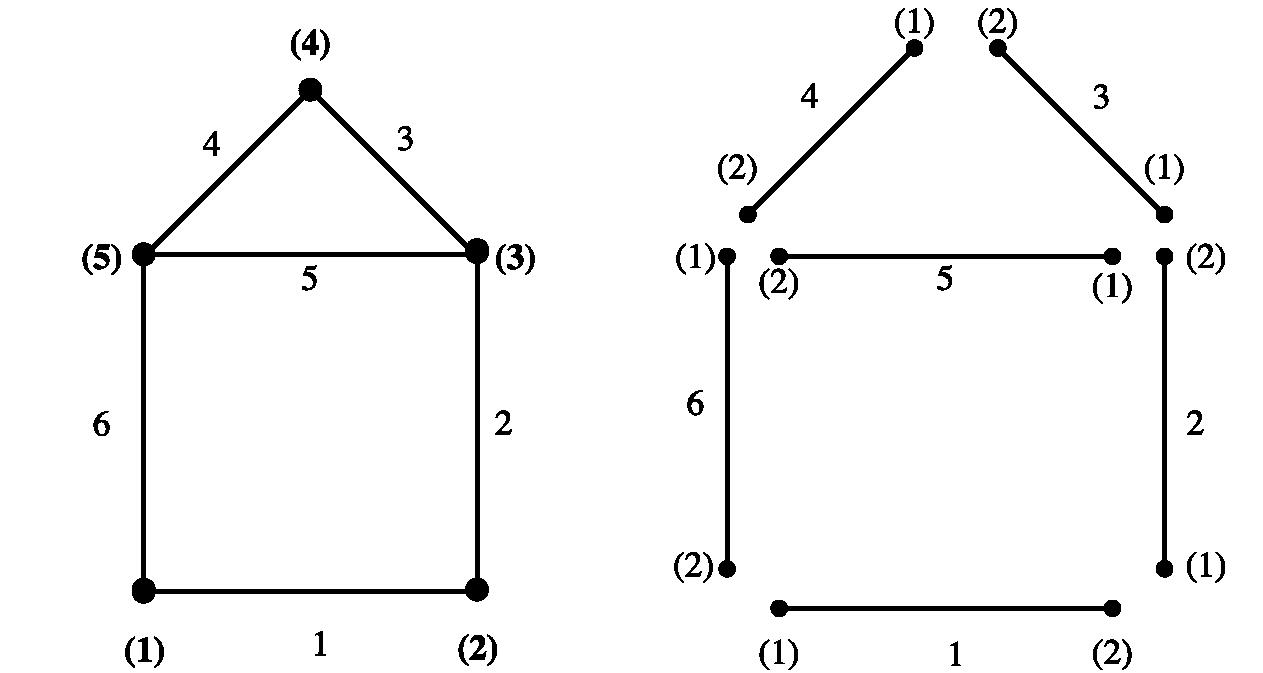
\includegraphics[scale=0.7]{figuras/malhaGen.pdf}	
	\caption{identificação global e local}
	\label{fig:malhaGenerica}
\end{figure}

\begin{figure}[!htb]
	\centering
	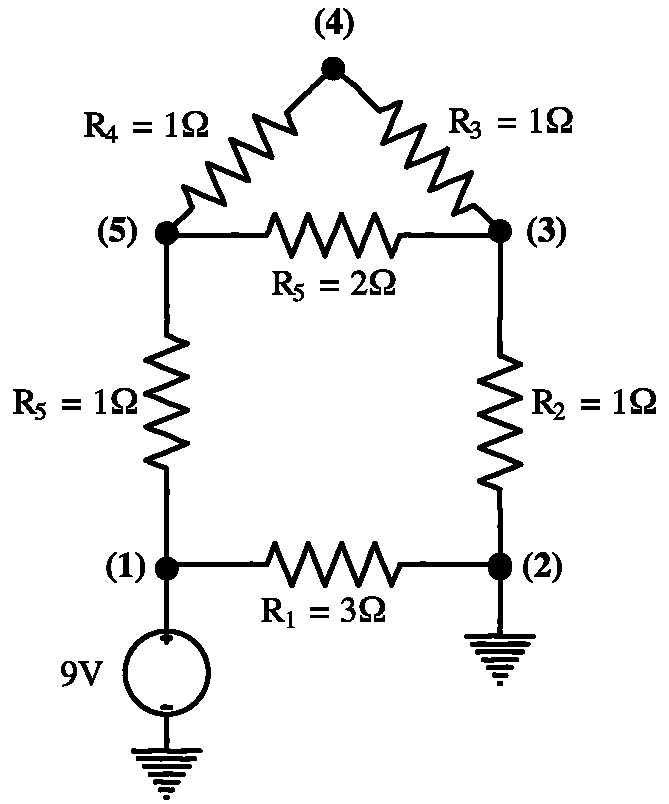
\includegraphics[scale=0.6]{figuras/circuito.pdf}
	\caption{Circuito puramente resistivo, um possível objeto de representação da malha da figura \ref{fig:malhaGenerica}}
	\label{fig:repMalhaGenerica}
\end{figure}

Na figura \ref{fig:malhaGenerica}, os elementos são identificados por números (sem parentesis) de $1$ a $6$. A identificação de cada nó, ou junção, é feita entre parêntesis. Na figura \ref{fig:malhaGenerica}$(a)$, em negrito, cada nó é relacionado à um identificador global, enquanto na figura \ref{fig:malhaGenerica}$(b)$, os nós possuem identificadores locais, relativos não ao conjunto total de nós, mas apenas aos nós de um dado elemento. Estes identificadores são necessários para a análise de um único elemento e em seguida para a montagem do sistema como um todo.

Fazendo a analogia com um pórtico, as forças que atuam sobre cada nó, podem ser definidas a partir dos deslocamento destes nós \cite[p. 3]{zien}. Esta relação é dada pela lei de Hooke simples, mostrada na equação \ref{eq:hooke1}, na qual as forças $Q_1$ e $Q_2$ sobre os nós de um elemento são dadas calculadas em função dos deslocamentos $u_1$ e $u_2$. A constante $A$ é a área do elemento, $E$ é o módulo de Young (Módulo de Elasticidade) e $l$ é o cumprimento do elemento \cite[p. 13]{desai}.

\begin{equation}
\label{eq:hooke1}
\left \{
\begin{tabular}{c}
$Q_1$ \\
$Q_2$
\end{tabular}       
\right \} =
\frac{AE}{l}
\begin{bmatrix}
1 & -1 \\
-1 & 1
\end{bmatrix}      
\left \{
\begin{tabular}{c}
$u_1$ \\
$u_2$
\end{tabular}       
\right \}            
\end{equation}


No circuito resistivo da figura \ref{fig:repMalhaGenerica}, a relação para um elemento é dada pela Lei de Ohm, na qual as correntes em cada nó, podem ser definidas à partir das tensões nos terminais do elemento. Na equação \ref{eq:ohm1}, $I_a$ e $V_a$ são respectivamente a corrente e a tensão no nó $a$ de um elemento, enquanto $R$ é a resistência do mesmo \cite[p. 7]{zien}.

\begin{equation}
\label{eq:ohm1}
\left \{
\begin{tabular}{c}
$I_1$ \\
$I_2$
\end{tabular}       
\right \} =
\frac{1}{R}
\begin{bmatrix}
1 & -1 \\
-1 & 1
\end{bmatrix}      
\left \{
\begin{tabular}{c}
$V_1$ \\
$V_2$
\end{tabular}       
\right \}            
\end{equation}

O padrão encontrado nas equações \ref{eq:hooke1} e \ref{eq:ohm1} pode ser generalizado para outros campos da engenharia, ciência e até mesmo administração e economia, desde que possam ser modelados por sistema de equações lineares \cite[p. 331]{burdenFaires}.

A questão a ser respondida é: Como analisar o efeito global de uma ação realizada em um conjunto limitado de nós? Por exemplo, como obter o potencial elétrico nos nós $3$, $4$ e $5$, da figura \ref{fig:repMalhaGenerica}, a partir da aplicação das tensões $9V$ e $0V$ nos nós $1$ e $2$ respectivamente? Como compilar os resultados locais  para o cálculo de grandezas secundárias, como a corrente ou potência elétrica em cada elemento, por exemplo? Estas questões serão respondidas nas duas subseções seguintes.


section{Equações do Elemento Discreto}

Se um fenômeno que atua sobre um dado elemento $e$ é modelado por um sistema de equações lineares,  pode ser representado em sua forma matricial como:

\begin{equation}
\label{eq:sisLinGen}
\{q^e\} = [K^e] \{u^e\} + \{f^e\}
\end{equation}

O vetor $q$ é conhecido ou parcialmente conhecido. Ele é geralmente uma grandeza secundária, calculada a partir da distribuição da grandeza primária $u$ desconhecida. A matriz $K$ é a matriz de coeficientes e determina como é feita a distribuição da grandeza $u$. No exemplo de estruturas, $K$ é a matriz de rigidez, $q$ é o conjunto de forças que atuam nos nós do elemento e $u$ é o deslocamento destes nós causados por estas forças. Para circuitos elétricos, $K$ relaciona as resistências do sistema, $q$ é a corrente no elemento, originada pela diferença de potencial $u$ em seus nós. O vetor $f$ é o estado inicial do elemento. Caso este estado seja de equilíbrio (sem torção inicial ou corrente residual, por exemplo), $f$ é igual a zero \cite[p. 7]{zien}.

As componentes de cada vetor da equação \ref{eq:sisLinGen} são relativas aos nós do elemento e a ordem da matriz $K$ é igual ao número de nós deste elemento. O número de nós de um elemento também é denominado \textbf{grau de liberdade} \cite[p. 5]{zien}. A equação \ref{eq:assembly} mostra a representação de um elemento com grau de liberdade  $m$. Se vista como uma matriz de adjacência, $K$ mostra como cada nó se relaciona com os demais. 

\begin{equation}
\label{eq:assembly}
\begin{tabular}{c c c}
$q^e = 
\left \{
\begin{tabular}{c}
$q^e_1$ \\
$q^e_2$ \\
\vdots \\
$q^e_m$
\end{tabular}       
\right \}$
\
$u^e = 
\left \{
\begin{tabular}{c}
$u_1$ \\
$u_2$ \\
\vdots \\
$u_m$
\end{tabular}       
\right \}   $
\
$K^e =
\begin{bmatrix}
K^e_{11}    & K^e_{12}  & \dots     & K^e_{1m} \\
K^e_{11}    & \ddots  & \   & \vdots \\
\vdots  & \vdots     & \    & \vdots \\
K^e_{m1}    & \dots   & \dots   & K^e_{mm} 
\end{bmatrix}    $      
\end{tabular} 
\end{equation}


Como pode ser visto na figura \ref{fig:malhaGenerica}$(b)$, cada elemento compartilha nós com seus vizinhos, de forma que, o resultado obtido no nó de um elemento deve ser compatível com os resultados obtidos nos outros elementos, para o mesmo nó. Esta condição de compatibilidade e equilíbrio será vista na subseção seguinte.

\section{Montagem do Sistema Global}

Para que uma ação local em um nó seja corretamente transmitida para os nós vizinhos, e dessa forma tenha seus efeitos refletidos em todo o sistema, é necessário relacionar todos os elementos e nós em um único sistema de equações. A equação \ref{eq:sisLinGen2} mostra um sistema global genérico. Sendo $n$ o número total de nós, $q$, $u$ e $f$ são vetores coluna de comprimento $n$ e $K$ é uma matriz quadrada de ordem $n$.

\begin{equation}
\label{eq:sisLinGen2}
\{q\} = [K] \{u\} + \{f\}
\end{equation}

A montagem do sistema \ref{eq:sisLinGen2} consiste no mapeamento dos sistemas elementares para um único sistema global e na aplicação das condições de equilíbrio pertinentes ao problema \cite[p. 5]{zien}.

No mapeamento, a matriz global de coeficientes pode ser vista como uma matriz de adjacência de todos os nós. Desta forma, ações locais sobre um elemento podem ser propagadas para os elementos vizinhos.
Enquanto nas equações elementares os nós são referenciados localmente, como na figura \ref{fig:malhaGenerica}$(b)$, no sistema global cada nó possui uma única referência, conforme a figura \ref{fig:malhaGenerica}$(a)$. As influências de diferentes elementos sobre um nó são somadas na matriz global, de forma que se tenha uma influência resultante.

O próximo passo é a aplicação da condição de equilíbrio para cada nó, conforme a lei que modela o problema. Para problemas de mecânica, por exemplo, a condição de equilíbrio dada pela 3ª lei de Newton diz que o somatório das forças em um ponto é igual a zero. Similarmente na análise de circuitos, a lei de Kirchoff diz que a soma das correntes que entram e saem de um nó também é igual a zero. A equação \ref{eq:somaForcas} mostra a aplicação da condição de equilíbrio no nó $a$.


\begin{equation}
\label{eq:somaForcas}
\sum_{e=1}^{m}{q_a^e = q_a^1 + q_a^2 + \dots = 0}
\end{equation}

Considerando que o estado inicial $f$ do corpo é nulo, o sistema \ref{eq:sisLinGen2} que possui $m$ nós e $n$ elementos, pode ser representado como 

\begin{equation}
\label{eq:equilibrio}
q =
\sum_{b=1}^{n}\sum_{e=1}^{m}{K_{ab}^e u_b = 0}
\end{equation}


\section{Atribuição das condições de Contorno}
A atribuição dos valores de contorno consiste na imposição dos valores preestabelecidos da variável $u$. No exemplo \ref{fig:repMalhaGenerica}, as condições de contorno são os valores da tensão $u$  impostos nos nós $1$ e $2$, como mostra a equação a seguir

\begin{equation}
\label{eq:condIni}
u = 
\left \{
\begin{tabular}{c}
$9V$ \\
$0V$ \\
$u_3$ \\
$u_4$ \\
$u_5$ \\
\end{tabular}       
\right \}   
\end{equation}

Com isso, a inserção de valores de contorno no sistema promove a redução do número de equações de equilíbrio do sistema apresentado em \ref{eq:equilibrio}, por meio da eliminação das linhas cujo valor de $u$ já foi especificado \cite[p. 5]{zien}.

\section{Exemplo: Associação de resistores}

A partir dos passos apresentados nas subseções acima, deve-se determinar os valores das tensões nós nós $3$, $4$ e $5$ à partir da diferença de potencial entre os nós $1$ e $2$.

O primeiro passo para a resolução do problema é a especificação das equações de cada elemento. Como é apresentado na equação \ref{eq:ohm1}, as correntes em cada nó de um elemento são dadas pelas diferenças de potencial destes nós. Com isso, para cada resistor, tem-se:

\begin{equation}
\label{eq:ohmMalha}
\begin{tabular}{l l}
$
e = 1:
\left \{
\begin{tabular}{l}
$I_1^1 = \frac{1}{3} (V_1^1 - V_2^1)$ \\
$I_2^1 = \frac{1}{3} (-V_1^1 + V_2^1)$
\end{tabular}       
\right .       
$
&
$
e = 2:
\left \{
\begin{tabular}{l}
$I_1^2 = V_1^2 - V_2^2$ \\
$I_2^2 = -V_1^2 + V_2^2$
\end{tabular}       
\right .       
$
\\ \\
$
e = 3:
\left \{
\begin{tabular}{l}
$I_1^3 = V_1^3 - V_2^3$ \\
$I_2^3 = -V_1^3 + V_2^3$
\end{tabular}       
\right .       
$
&
$
e = 4:
\left \{
\begin{tabular}{l}
$I_1^4 = V_1^4 - V_2^4$ \\
$I_2^4 = -V_1^4 + V_2^4$
\end{tabular}       
\right .       
$
\\ \\
$
e = 5:
\left \{
\begin{tabular}{l}
$I_1^5 = \frac{1}{2} (V_1^5 - V_2^5)$ \\
$I_2^5 = \frac{1}{2} (-V_1^5 + V_2^5)$
\end{tabular}       
\right .       
$
&
$
e = 6:
\left \{
\begin{tabular}{l}
$I_1^6 = V_1^6 - V_2^6$ \\
$I_2^6 = -V_1^6 + V_2^6$
\end{tabular}       
\right .       
$                    
\end{tabular}               
\end{equation}

Uma vez definidas as equações de cada elemento é feita a montagem do sistema global. Conforme dito anteriormente, a etapa de montagem consiste no mapeamento da numeração local dos nós para um sistema de numeração global. Analisando a figura \ref{fig:malhaGenerica}$(b)$, é possível notar que os nós $1$ e $2$ do elemento $2$, por exemplo, são os nós $2$ e $3$ do sistema global apresentado na figura \ref{fig:malhaGenerica}$(a)$. A tabela \ref{tab:mapLG} relaciona os identificadores locais e seus equivalentes no sistema global.

\begin{table} 
	\centering
	\begin{tabular}{|c|c|}  
		\hline
		\textbf{Identificação Local} 
		& \textbf{Identificação Global} \\  
		\hline
		$e_1^1, e_2^6$ 
		& $1$ \\
		\hline
		$e_2^1, e_1^2$
		& $2$  \\
		\hline
		$e_2^2, e_1^3, e_1^5$
		& $3$ \\
		\hline
		$e_2^3, e_1^4$
		& $4$  \\
		\hline
		$e_2^4, e_2^5, e_1^6$
		& $5$  \\        
		\hline
	\end{tabular}
	\caption{Mapeamento dos identificadores locais do circuito da figura \ref{fig:malhaGenerica}}
	\label{tab:mapLG}
\end{table}

A equação \ref{eq:mapE1} a seguir, apresenta o mapeamento do elemento $1$ e em seguida, na equação \ref{eq:mapE2}, é incluído o mapeamento do elemento $2$.  

\begin{equation}
\label{eq:mapE1}
\left \{
\begin{tabular}{c}
$I_1$ \\
$I_2$ \\
$I_3$ \\
$I_4$ \\
$I_5$          
\end{tabular}       
\right \}
=
\begin{bmatrix}
\frac{1}{3} & \frac{-1}{3}  & 0 & 0 & 0 \\
\frac{-1}{3} & \frac{1}{3}  & 0 & 0 & 0 \\
0 & 0 & 0 & 0 & 0 \\
0 & 0 & 0 & 0 & 0 \\
0 & 0 & 0 & 0 & 0 \\
\end{bmatrix} 
\left \{
\begin{tabular}{c}
$V_1$ \\
$V_2$ \\
$V_3$ \\
$V_4$ \\
$V_5$          
\end{tabular}       
\right \}	                     
\end{equation}

\begin{equation}
\label{eq:mapE2}
\left \{
\begin{tabular}{c}
$I_1$ \\
$I_2$ \\
$I_3$ \\
$I_4$ \\
$I_5$          
\end{tabular}       
\right \}
=
\begin{bmatrix}
\frac{1}{3} & \frac{-1}{3}  & 0 & 0 & 0 \\
\frac{-1}{3} & \frac{1}{3}+1  & -1 & 0 & 0 \\
0 & -1 & 1 & 0 & 0 \\
0 & 0 & 0 & 0 & 0 \\
0 & 0 & 0 & 0 & 0 \\
\end{bmatrix} 
\left \{
\begin{tabular}{c}
$V_1$ \\
$V_2$ \\
$V_3$ \\
$V_4$ \\
$V_5$          
\end{tabular}       
\right \}	                     
\end{equation}

Todas as contribuições em um dado nó, devem ser consideradas. Por este motivo, quando houverem influências de diferentes elementos sobre um nó, as mesmas devem ser somadas no sistema global. A equação \ref{eq:mapFinal} apresenta o sistema global final, com as contribuições de todos os $6$ elementos.

\begin{equation}
\label{eq:mapFinal}
\left \{
\begin{tabular}{c}
$I_1$ \\
$I_2$ \\
$I_3$ \\
$I_4$ \\
$I_5$          
\end{tabular}       
\right \}
=
\begin{bmatrix}
\frac{1}{3} & \frac{-1}{3}  & 0 & 0 & 0 \\
\frac{-1}{3} & \frac{4}{3}  & -1 & 0 & 0 \\
0 & -1 & 2 & -1 & 0 \\
0 & 0 & -1 & 2 & -1 \\
0 & 0 & 0 & -1 & 1 \\
\end{bmatrix} 
\left \{
\begin{tabular}{c}
$V_1$ \\
$V_2$ \\
$V_3$ \\
$V_4$ \\
$V_5$          
\end{tabular}       
\right \}	                     
\end{equation}


% ---



\chapter{Método dos elementos finitos em 2 dimensões}
\label{sec:fem2d}
Neste capítulo será apresentada a solução de um modelo de elementos finitos. O exemplo desenvolvido foi adaptado do exemplo $6.1$ de \citeonline{sadiku}. Deseja-se saber o valor do potencial elétrico nos pontos $a$ e $b$ da placa submetida a uma diferença de potencial de $10V$, como mostra a figura \ref{fig:exemplo}{a}.

\begin{figure}%
	\centering
	\subfloat[Geometria do problema]{{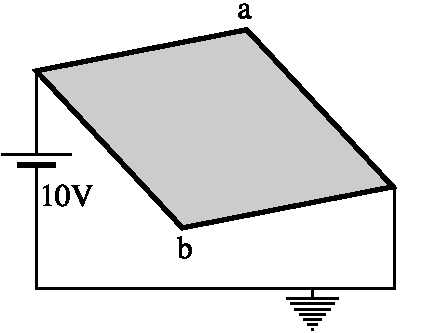
\includegraphics[scale=0.7]{figuras/exemploG.pdf} }}%
	\qquad
	\subfloat[Triangulação do problema]{{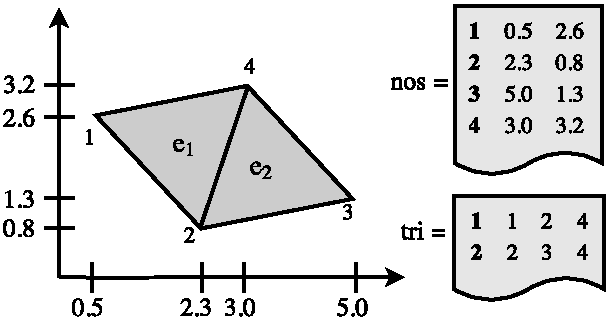
\includegraphics[scale=0.7]{figuras/exemplo.pdf} }}%
	\caption{Exemplo do FEM em 2 dimensões}%
	\label{fig:exemplo}%
\end{figure}

O primeiro passo consiste em realizar a triangulação da malha. Uma possibilidade de malha é apresentada na figura \ref{fig:exemplo}[b]. A estrutura de dados $tri$ contém a informação sobre quais vértices formam cada elemento enquanto a estrutura $nos$ possui as coordenadas de todos os vértices da geometria do problema. 

O passo seguinte é a definição da função de interpolação. A aproximação da distribuição do potencial num dado elemento pode ser feita por uma função linear, como mostra a equação \ref{eq:interpEx}. Desta forma, os valores de $V$ em cada nó podem ser obtidos pelo sistema de equações \ref{eq:interpNoEx}

\begin{equation}
\label{eq:interpEx}
\tilde{V^e} = a^e + b^e x + c^e y
\end{equation}

\begin{equation}
\label{eq:interpNoEx}
\begin{Bmatrix}
\tilde{V^e_1}  \\
\tilde{V^e_2} \\
\tilde{V^e_3}
\end{Bmatrix}
=
\begin{bmatrix}
1 & x_1 & y_1 \\
1 & x_2 & y_2 \\
1 & x_3 & y_3
\end{bmatrix}
\begin{Bmatrix}
a \\
b \\
c
\end{Bmatrix}
\end{equation}

Deseja-se então resolver o problema encontrando os valores dos coeficientes $a$, $b$ e $c$ que fazem a aproximação de $V$. Dada a simplicidade o sistema ele pode ser resolvido invertendo-se a matriz por meio do cálculo dos determinantes e cofatores. Os valores da transposta da matriz de cofatores são dados na equação \ref{eq:cof} e o determinante na equação \ref{eq:det}. A equação \ref{eq:subs} contém a substituição na equação \ref{eq:interpEx} dos valores dos coeficientes calculados.

\begin{equation}
\label{eq:cof}
cof(A^e)^T
=
\begin{bmatrix}
(x_2y_3 - x_3y_2) & (x_3y_1 - x_1y_3) & (x_1y_2 - x_2y_1) \\
(y_2 - y_3) & (y_3 - y_1) & (y_1 - y_2) \\
(x_3 - x_2) & (x-1 - x_3) & (x_2 - x_1)
\end{bmatrix}
\end{equation}

\begin{equation}
\label{eq:det}
det(A^e)
=
(x_1y_2 - x_2y_1)+
(x_3y_1 - x_1y_3)+
(x_2y_3 - x_3y_2)
\end{equation}

\begin{equation}
\label{eq:subs}
\tilde{V^e} = 
\begin{Bmatrix}
1 & x & y
\end{Bmatrix}
\begin{Bmatrix}
a \\ b \\ b
\end{Bmatrix}
= \begin{Bmatrix}
1 & x & y
\end{Bmatrix}
\frac{cof(A^e)^T}{det(A^e)}
\begin{Bmatrix}
\tilde{V^e_1}  \\
\tilde{V^e_2} \\
\tilde{V^e_3}
\end{Bmatrix}
=
\sum_{j=1}^{3}{N_j^e (x, y) \tilde{V}_j^e}
\end{equation}

Obtidas as funções de interpolação $N^e$, a próxima etapa consiste  na montagem do sistema de equações do problema, começando pela definição das matrizes elementares. A distribuição do potencial é modelada pela equação de Laplace $\nabla^2 V = 0$. Substituindo esta equação em \ref{eq:res2} e adotando-se o método de Galerkin, tem-se a integral \ref{eq:lapPon}.

\begin{equation}
\label{eq:lapPon}
\iint_{}{N^e_i \nabla^2 V^e dx dy} = R^e_i \qquad i = 1,2,3.
\end{equation}  

Aplicando a integração por partes fazendo $u = N$ e $dv = nabla^2 V$, tem-se como resultado da relação $\int u dv = uv - \int vdu$ a equação \ref{eq:posParte}.

\begin{equation}
\label{eq:posParte}
\iint_{}{\nabla V^e \nabla N^e_i dx dy} = R^e_i \qquad i = 1,2,3.
\end{equation} 

Substituindo $V^e$ por sua aproximação obtida em (\ref{eq:subs}) obtém-se a fórmula da matriz elementar nas equações \ref{eq:integEl} e \ref{eq:matEl}.

\begin{equation}
\label{eq:integEl}
\iint_{}{ \sum_{j=1}^{3}{\nabla N_j^e \tilde{V}_j^e} \nabla N^e_i dx dy} 
=
\sum_{j=1}^{3}\iint_{}{\left(\nabla N^e_i \nabla N_j^e \right)  \tilde{V}_j^e dx dy}
= R^e_i \qquad i = 1,2,3.
\end{equation} 

\begin{equation}
\label{eq:matEl}
K^e_{ij} 
= 
\iint_{}{\left(\nabla N^e_i \nabla N_j^e \right)  dx dy}
\end{equation} 

De forma a agilizar os cálculos das matrizes elementares define-se na equação \ref{eq:PQA}  a partir dos elementos das equações \ref{eq:cof} e \ref{eq:det} as variáveis $P$, $Q$ e $A$. $P$ e $Q$ são obtidas a partir das simplificações nos cálculos e $A$ é a área do triângulo.  A equação \ref{eq:usoSimp} mostra como os coeficientes podem ser calculados após a simplificação

\begin{equation}
\label{eq:PQA}
\begin{matrix}
P_1 = (y_2 - y_3) & P_2 = (y_3 - y_1) & P_3 = (y_1 - y_1) \\
Q_1 = (x_3 - x_2) & Q_2 = (x_1 - x_3) & Q_3 = (x_2 - x_1) \\
\ & A = \frac{1}{2}(P_2Q_3 - P_3Q_2) & \
\end{matrix}
\end{equation}

\begin{equation}
\label{eq:usoSimp}
K^e_{ij} 
= 
\frac{1}{4A}(P_iP_j + Q_iQ_j)
\end{equation}

As matrizes dos elementos e a matriz global são apresentadas nas equações \ref{eq:exMatel} e \ref{eq:exMatG}. Após a definição das matrizes elementares é realizado o mapeamento de seus coeficientes para a matriz global. Enquanto a matriz elementar é da ordem do número de nós do elemento, a matriz global de coeficientes é da ordem do número de nós da malha. O processo de mapeamento é detalhado no apêndice \ref{sec:SED}.

\begin{equation}
\label{eq:exMatel}
K^1 = 
\begin{pmatrix}
0,560 &	-0,285 &	-0,274 \\
-0,285 &	0,592 &	-0,3066\\
-0,274 &	-0,306 &	0,580\\
\end{pmatrix}
\
K^2 =
\begin{pmatrix} 
0,620 &	-0,257 &	-0,362\\
-0,257 &	0,509 &	-0,252\\
-0,362 &	-0,252 &	0,615
\end{pmatrix}
\end{equation}

\begin{equation}
\label{eq:exMatG}
K = 
\begin{pmatrix}
0,560 &	-0,285 &	0&	-0,274\\
-0,285&	1,213&	-0,257&	-0,669\\
0&	-0,257&	0,509&	-0,252\\
-0,274&	-0,669&	-0,252&	1,195
\end{pmatrix}
\end{equation}

A atribuição dos valores de contorno consiste na redução da ordem na matriz \ref{eq:exMatG} por meio da eliminação dos graus de liberdade (nós) com valores pré estabelecidos (contorno). As equações \ref{eq:exMatCont1} e \ref{eq:exMatCont2} exibem o sistema reduzido e a solução.

\begin{equation}
\label{eq:exMatCont1}
\begin{pmatrix}
0,560 &	-0,285 &	0&	-0,274\\
-0,285&	1,213&	-0,257&	-0,669\\
0&	-0,257&	0,509&	-0,252\\
-0,274&	-0,669&	-0,252&	1,195
\end{pmatrix}
\begin{Bmatrix}
10 \\
V^2\\
0\\
V^4
\end{Bmatrix}
=
\begin{Bmatrix}
0\\
0\\
0\\
0
\end{Bmatrix}
\end{equation}


\begin{equation}
\label{eq:exMatCont2}
\begin{pmatrix}
-0.285  & -0.257\\
-0.274 &  -0.252\\
\end{pmatrix}
\begin{Bmatrix}
V^2\\
V^4
\end{Bmatrix}
=
\begin{Bmatrix}
 2.858\\
 2.741
\end{Bmatrix}
\Rightarrow
\begin{Bmatrix}
V^2 \\
V^4
\end{Bmatrix}
=
\begin{Bmatrix}
5.241\\
5.227
\end{Bmatrix}
\end{equation}

\end{apendicesenv}
% ---

\end{document}
